\documentclass[AMA,STIX1COL]{WileyNJD-v2}

\articletype{Research Article}%

\received{}
\revised{}
\accepted{}

\raggedbottom

\usepackage{amsfonts}
\usepackage[fleqn,reqno]{amsmath}
\usepackage{amssymb}
\usepackage[titletoc]{appendix}
\usepackage{enumitem}
\usepackage{filecontents}
\usepackage[top=1.2in,bottom=1.2in,left=1in, right=1in]{geometry}
\usepackage{graphics}
\usepackage{lineno}
%\usepackage{showkeys} %To see the labels for now.  Will remove later
\usepackage{pgfplots}
\usepackage{tikz}
\usepackage{todonotes}

\usetikzlibrary{arrows}


%%%%%%  pdftex  %%%%%%%%%%%%%%%%%%%%%%%%%%%%%%%%%%%%%%%%%%%%%%%%%%%%%%
\usepackage[pagebackref=false,bookmarks=false]{hyperref} 

\hypersetup{
  bookmarksnumbered=true,
  bookmarksopen=false,
  hypertexnames=false,      
  breaklinks=true,          
  unicode=false,
  pdffitwindow=true,        
  pdfnewwindow=true,        
  colorlinks=true,         
  linkcolor=dblue,
  anchorcolor=red,
  citecolor=dorange,
  filecolor=magenta,
  urlcolor=dblue,
  pdfstartview = FitH,
  pdfkeywords = {},
  pdfcreator = {LaTeX with hyperref package}
}

\newcommand{\bd}{{\partial}}
\newcommand{\cc}{{\mathbf{c}}}
\newcommand{\DD}{{\mathcal{D}}}
\newcommand{\eeta}{{\boldsymbol\eta}}
\newcommand{\ff}{{\mathbf{f}}}
\newcommand{\grad}{{\nabla}}
\newcommand{\llambda}{{\boldsymbol\lambda}}
\newcommand{\nn}{{\mathbf{n}}}
\newcommand{\NN}{{\mathcal{N}}}
\newcommand{\pderiv}[2]{\frac{\partial #1}{\partial #2}}
\newcommand{\rr}{{\mathbf{r}}}
\newcommand{\RR}{{\mathbb{R}}}
\renewcommand{\ss}{{\mathbf{s}}}
\newcommand{\ssigma}{{\boldsymbol\sigma}}
\newcommand{\uu}{{\mathbf{u}}}
\newcommand{\UU}{{\mathbf{U}}}
\newcommand{\vv}{{\mathbf{v}}}
\newcommand{\xx}{{\mathbf{x}}}
\newcommand{\xxi}{{\boldsymbol{\xi}}}
\newcommand{\yy}{{\mathbf{y}}}

\begin{document}

\title{Stable and contact-free time stepping for dense rigid particle
suspensions}

\author[1]{Lukas Bystricky}

\author[2]{Sachin Shanbhag}

\author[2,3]{Bryan Quaife*}

\authormark{Bystricky \textsc{et al}}

\address[1]{\orgdiv{Department of Mathematics},
\orgname{KTH}, \orgaddress{\state{Stockholm},\country{Sweden}}}

\address[2]{\orgdiv{Department of Scientific Computing},
\orgname{Florida State University}, \orgaddress{\state{Florida},
\country{USA}}}

\address[3]{\orgdiv{Geophysical Fluid Dynamics Institute},
\orgname{Florida State University}, \orgaddress{\state{Florida},
\country{USA}}}

\corres{Bryan Quaife, Department of Scientific Computing, Florida State
University. \email{bquaife@fsu.edu}}

%\presentaddress{This is sample for present address text this is sample for present address text}

\abstract[Summary]{We consider suspensions of rigid bodies in a
two-dimensional viscous fluid. Even with high-fidelity numerical
methods, unphysical contact between particles occurs because of spatial
and temporal discretization errors.  We apply the method of Lu et
al.~[{\em Journal of Computational Physics}, {\bf 347}:160--182, 2017]
where overlap is avoided by imposing a minimum separation distance.  In
its original form, the method discretizes interactions between different
particles explicitly.  Therefore, to avoid stiffness, a large minimum
separation distance is used.  In this paper, we extend the method of Lu
et al.~by treating all interactions implicitly.  This new time stepping
method is able to simulate dense suspensions with large time step sizes
and a small minimum separation distance.  The method is tested on
various unbounded and bounded flows, and rheological properties of the
resulting suspensions are computed.}

\keywords{Stokes flow, Boundary integral method, Rigid body suspensions,
Collision handling, Rheology}

\jnlcitation{\cname{%
\author{L.~Bystricky}, 
\author{S. Shanbhag}, 
\author{B. Quaife}} (\cyear{2018}), 
\ctitle{Stable and contact-free time stepping for dense rigid particle
  suspensions},
\cjournal{Int J Numer Meth Fl},
\cvol{}.}

\maketitle

%\footnotetext{\textbf{Abbreviations:} ANA, anti-nuclear antibodies; APC, antigen-presenting cells; IRF, interferon regulatory factor}

\section{Introduction}\label{s:intro}
Dispersions of rigid fibers particles are used in composite materials to
tune mechanical, thermal, and electrical properties. Typically, these
materials are processed in the melt or liquid suspension state via
operations like injection molding, extrusion, casting, etc. It is
important to model particle suspensions for two reasons: (i) the
distribution and orientation of the particles, which determines the
properties of the composite material, are governed by the flow history
during processing, and (ii) the rheological properties of the
suspension, which influence the flow behavior, in turn, depend on the
size, shape, distribution, and orientation of the
particles~\cite{larsoncf}.

The theory of rigid rods in flowing fluids was pioneered by
Jeffery~\cite{Jeffery1922} who analyzed the motion of a single
spheroidal particle sheared in a Newtonian solvent. At a given shear
rate $\dot{\gamma}$, he observed that rods of length $\ell$ and diameter
$d$ underwent periodic motion with a period $\pi/(2|\dot{\gamma}|)
(\lambda + 1/\lambda)$, where $\lambda = \ell/d$ is the aspect ratio.
The period increases with $\lambda$, and when $\lambda \gg 1$, a
particle exhibiting a ``Jeffery's orbit" stays aligned with the flow
direction most of the time, before abruptly spinning through a
half-revolution. In the dilute regime (number of rods/unit volume $\nu <
1/\ell^3$), trajectories of elongated fibers of different shapes, such
as cylinders, can be quantitatively described via Jeffery's orbits once
corrections are made for particle shape~\cite{Bretherton1962}.

As $\nu$ increases, interactions between rods become significant.
Analytical solutions become intractable, and computer simulations have
to be resorted to. In these simulations, the distribution of particle
orientations is modeled either implicitly or explicitly. In the
\emph{implicit} approach, individual particles are not explicitly
represented; instead it relies on averages of second- and fourth-order
orientation tensors. Fluid flow equations (Stokes or Navier-Stokes) are
coupled with evolution equations for the orientation tensors. In order
to solve the resulting equations, models for interaction between
particles and closure approximations have to be specified
externally~\cite{Advani1987, Advani1990, Ferec2014, Perez2017}. This is
in contrast to direct numerical simulations where individual particles
are \emph{explicitly} represented. Typically, rod-like particles are
modeled as prolate ellipsoids~\cite{Ausias2006}, a set of connected
beads~\cite{Yamamoto1996, Joung2001},
rods~\cite{Schmid2000,Lindstroem2007}, or a slender body ($\ell \gg
d$)~\cite{Fan1998, Rahnama1995, tor-she2004, tor-gus2006, gus-tor2009},
with suitable first-order corrections to account for finite width. Over
the years, in addition to long-range hydrodynamic interaction, these
models have been supplemented with detailed physics including
short-range lubrication, mechanical contact, and frictional
forces~\cite{Sundararajakumar1997, Lindstroem2008}.

In this work, we develop and test tools for two-dimensional direct
numerical simulations of rigid bodies suspended in a viscous fluid.  We
do not make any rigid body assumptions, but rather fully resolve the
fiber shape.  To perform the simulations, we use a boundary integral
equation (BIE) since it resolves the complex geometry by reducing the
set of unknowns to the one-dimensional closed curves that form the fluid
boundary.  Moreover, our BIE fluid solver achieves high-order accuracy.
The governing Stokes equations prohibit contact between particles,
however, because of numerical errors, without additional techniques,
rigid bodies often come into contact or even overlap.  Therefore, we use
a globally implicit time stepping method coupled with a contact
algorithm.  In this manner, rigid particles can come very close to one
another, but guarantees that contact is avoided without introducing
significant stiffness.  This contact algorithm results in a flow that is
not reversible, and we compute and analyze this error.  Finally, we
compute rheological and statistical properties of the fluid and
particles to better understand the dispersion of fibers in composite
materials.

%Dispersions of particulate rods or fibers are used in composite
%materials to tune mechanical, thermal, and electrical properties.
%Typically, these materials are processed in the melt or liquid
%suspension state via operations like injection molding, extrusion,
%casting, etc. It is important to model fiber suspensions for two
%reasons: (i) the distribution and orientation of the fibers, which
%determines the properties of the composite material, are governed by the
%flow history during processing, and (ii) the rheological properties of
%the suspension, which influence the flow behavior, in turn, depend on
%the size, shape, distribution, and orientation of the
%fibers~\cite{larsoncf}.
%
%The theory of rigid fibers in flowing fluids was pioneered by
%Jeffery~\cite{Jeffery1922} who analyzed the motion of a single
%spheroidal particle sheared in a Newtonian solvent. At a given shear
%rate $\dot{\gamma}$, he observed that fibers of length $\ell$ and
%diameter $d$ underwent periodic motion with a period $\pi/(2|\dot{\gamma}|)
%(\lambda + 1/\lambda)$, where $\lambda = \ell/d$ is the aspect ratio.
%The period increases with $\lambda$, and when $\lambda \gg 1$, a
%particle exhibiting a ``Jeffery's orbit" stays aligned with the flow
%direction most of the time, before abruptly spinning through a
%half-revolution. In the dilute regime (number of rods/unit volume $\nu <
%1/\ell^3$), trajectories of elongated fibers of different shapes, such
%as cylinders, can be quantitatively described via Jeffery's orbits once
%corrections are made for particle shape~\cite{Bretherton1962}.
%
%As $\nu$ increases, interactions between fibers become significant.
%Batchelor extended Jeffery's theory for multiple particles, by relating
%the average stress tensor, $\ssigma$, to the distribution of fiber
%orientation $\mathbf{p}$, and the deformation tensor $\mathbf{D} =
%(\nabla \mathbf{u} + \nabla \mathbf{u}^\intercal)/2$. Assuming purely
%hydrodynamic interactions between fibers, and a slender body
%approximation ($\lambda \gg 1$)~\cite{Batchelor1970, Batchelor1970a,
%Doi1978, Dinh1984, Shaqfeh1990},
%\begin{align}
%  \ssigma = 2 \mu \mathbf{D} + \nu \zeta 
%    \langle \mathbf{p p p p} \rangle : \mathbf{D},
%\label{eqn:batchelor}
%\end{align}
%where $\mu$ is the solvent viscosity, and $\zeta$ is a drag
%coefficient~\cite{Batchelor1971} that depends on the size and
%concentration of the particles, and the solvent viscosity. The ensemble
%average $\langle \cdot \rangle = \int \cdot \,
%\psi(\mathbf{p})\,d\mathbf{p}$ represents a weighted average over the
%probability distribution of fiber orientations $\psi(\mathbf{p})$. 
%
%In computer simulations, the fiber orientation distribution is modeled
%implicitly or explicitly. In the \emph{implicit} approach, individual
%fibers are not explicitly represented; instead it relies on averages of
%second- and fourth-order fiber orientation tensors, $\langle \mathbf{p
%p} \rangle$ and $\langle \mathbf{p p p p} \rangle$. Fluid flow equations
%(Stokes or Navier-Stokes) are coupled with evolution equations for the
%fiber orientation tensors. In order to solve the resulting equations,
%fiber interaction models and closure approximations have to be specified
%externally~\cite{Advani1987, Advani1990, Ferec2014, Perez2017}. This is
%in contrast to direct numerical simulations where individual fibers are
%\emph{explicitly} represented. Typically, fibers are modeled as
%prolate ellipsoids~\cite{Ausias2006}, a set of connected
%beads~\cite{Yamamoto1996, Joung2001}, rods~\cite{Schmid2000,
%Lindstroem2007}, or a slender body ($\ell \gg d$)~\cite{Fan1998,
%Rahnama1995, tor-she2004, tor-gus2006, gus-tor2009}, with suitable
%first-order corrections to account for finite width. Over the years, in
%addition to long-range hydrodynamic interaction, these models have been
%supplemented with detailed physics including short-range lubrication,
%mechanical contact, and frictional forces~\cite{Sundararajakumar1997,
%Lindstroem2008}.
%
%In the semi-dilute regime, $1/\ell^3 \ll \nu \ll 1/d\ell^2$, fiber
%rotation is hindered; however, it is found that the statistical
%properties are not significantly altered from the dilute
%regime~\cite{larsoncf}.  Hydrodynamic interactions between particles
%dominate the response, and contacts between fibers are rare. Batchelor's
%theory, suitably modified for multibody hydrodynamic
%interactions~\cite{Shaqfeh1990, Mackaplow1996}, describes the
%empirically observed increase in shear viscosity as a function of $\nu$
%reasonably well~\cite{Stover1992, Bibbo1987, Petrich2000}. The
%contribution of the fibers to the steady shear viscosity is relatively
%modest in non-Brownian suspensions. This is especially true for high
%aspect ratio fibers which rotate and align along the flow direction, and
%contribute to the viscosity only during the occasional
%tumble~\cite{larsoncf}.  Thus, the success of theory and computer models
%in predicting the viscosity change in the semi-dilute regime does not
%automatically validate the underlying fiber interaction model. Indeed
%fiber-fiber interactions are more sensitively reflected in other
%viscometric functions such as first normal stress difference, and
%distribution of orientations as reflected in, for example, the
%dispersion of Jeffery's orbits~\cite{Lindstroem2009}.
%
%Once the concentration increases beyond $\nu \approx 1/d\ell^2$, the
%suspension enters the concentrated regime. Here, excluded volume
%interactions become important and isotropic packing becomes increasingly
%difficult. In this regime, Batchelor's slender body theory and
%constitutive relation~\eqref{eqn:batchelor} are no longer valid as
%mechanical contacts between fibers start to dominate the response. When
%these mechanical interactions are explicitly accounted for, computer
%models are able to reproduce a nonzero first normal stress difference
%that is observed in experiments~\cite{Sundararajakumar1997, Ausias2006,
%Lindstroem2008}. Unlike the dilute and semi-dilute regimes, equation
%\eqref{eqn:batchelor} can no longer be used to estimate rheological
%properties. Instead, stresses in the suspension have to be computed by
%directly summing the forces acting on the fibers~\cite{Ausias2006,
%Lindstroem2008}.
%
%In this work, we develop and test tools for two-dimensional direct
%numerical simulations of rigid bodies suspended in a viscous fluid.  We
%do not make any rigid body assumptions, but rather fully resolve the
%fiber shape.  To perform the simulations, we use a boundary integral
%equation (BIE) since it resolves the complex geometry by reducing the
%set of unknowns to the one-dimensional closed curves that form the fluid
%boundary.  Moreover, our BIE fluid solver achieves high-order accuracy.
%The governing Stokes equations prohibit contact between particles,
%however, because of numerical errors, without additional techniques,
%rigid bodies often come into contact or even overlap. Therefore, we
%apply a contact algorithm that allows rigid particles to come very close
%to one another, but guarantees that contact is avoided without
%introducing significant stiffness.  In addition to computing fiber
%trajectories, we compute rheological and statistical properties of the
%fluid and particles to better understand the dispersion of fibers in
%composite materials.

\paragraph{Contributions} When deformable bodies, such as vesicles, approach
one another, the pressure in the lubrication region between the bodies
causes the membrane interfaces to flatten and this creates a natural
minimum separation distance~\cite{lac-mor-bar2007}.  However, for rigid
body suspensions, the inability to deform results in bodies coming much
closer together, and numerical errors can easily cause unphysical
overlap between particles.  To avoid overlap, Lu et al.~\cite{Lu2017}
developed a contact algorithm that guarantees a minimum separation
distance between bodies and used a {\em locally implicit} time stepping
method that only treats inter-body interactions implicitly.  That is, if
$\uu_{ij}$ is the velocity of body $i$ induced by body $j$, then the
locally implicit time stepping method is
\begin{align*}
  \frac{\xx_i(t + \Delta t) -  \xx_i(t)}{\Delta t} = 
    \uu_{ii}(t+\Delta t) + \sum_{j \neq i} \uu_{ij}(t),
\end{align*}
where $\xx_i$ is the center of the $i^{\mathrm{th}}$ body.  By treating
the interactions between different bodies explicitly, the minimum
separation distance must be kept sufficiently large to avoid a small
time step restriction due to stiffness---a typical minimum separation
distance is $\mathcal{O}(1)$ arclength spacings.

Our main contributions are extending the time stepping strategy
introduced for vesicle suspensions~\cite{Quaife2014} to rigid body
suspensions, analyzing the rheological properties of the suspensions,
and characterizing the loss of reversibility caused by the contact
algorithm.  The time stepping strategy we present is in line with
previous work of one of the authors~\cite{Quaife2014}.  The time
stepping method is {\em globally implicit} and discretizes all
interactions semi-implicitly
\begin{align*}
  \frac{\xx_i(t + \Delta t) -  \xx_i(t)}{\Delta t} = 
    \uu_{ii}(t+\Delta t) + \sum_{j \neq i} \uu_{ij}(t+\Delta t).
\end{align*}
With this modification, we are able to perform simulations with much
smaller and more physical minimum separation distances without
introducing excessive stiffness---we present results with a minimum
separation distance of $\mathcal{O}(10^{-2})$ arclength spacings.

While maintaining a minimum separation distance is important for stable
simulations, the contact algorithm developed by Lu et al.~introduces
artificial forces that shift bodies onto different streamlines, and this
breaks the reversibility of the Stokes equations.  We examine the effect
of the contact algorithm on the reversibility of the flow.  Finally, we
use our new time stepping to examine the rheological properties of dense
rigid body suspensions with small minimum separation distances.  In
particular, we compute the effective shear viscosity of a suspension of
rigid bodies in a Couette device, examine the alignment angle of
elliptical bodies of varying area fraction and aspect ratio, and compare
the results to analytical Jeffery's orbits.

\paragraph{Limitations} The main limitation is that the method is
developed in two dimensions.  By limiting ourselves to two dimensions,
we are able to perform simulations of denser suspensions  than would be
possible in three dimensions.  However, the algorithms we present have
been developed in three dimensions including boundary integral equation
methods and fast summation methods~\cite{cor-gre-rac-vee2017,
kli-tor2014, kli-tor2016}.  The most challenging algorithms to extend to
three dimensions include efficient preconditioners and a suspension
space-time interference volume that integrates a four-dimensional domain
($3$ space dimensions and $1$ time dimension).

Another limitation is that we only consider elliptical rigid bodies
whose minor and major axis differ by a factor of no more than six.
However, in many applications, the aspect ratio of slender bodies is at
least an order of magnitude larger.  Our formulation is valid for any
two-dimensional geometry with a smooth boundary, but the resolution must
be sufficiently large to resolve the geometry, layer potentials, and
density functions.

\paragraph{Related work} Rather than presenting an exhaustive list of
work related to particulate suspensions in viscous fluids, we focus on
literature related to BIEs and time stepping for rigid body suspensions.
A more complete overview of BIEs for particulate suspensions can be
found in the texts~\cite{Pozrikidis1992, Guazzelli2011, Karrila1991}.
Our work draws heavily from methods developed for simulating
two-dimensional vesicle suspensions~\cite{Quaife2014, Quaife2015,
qua-bir2016, Rahimian2010, Lu2017}.  

We represent the velocity as a completed double-layer potential
representation~\cite{Power1987, Power1993, Karrila1989} that is
discretized with high-order quadrature and solved iteratively with
GMRES~\cite{Saad1986}.  By using a double-layer potential, a second-kind
integral equation needs to be solved.  Upon discretization, the required
number of GMRES iterations is mesh-independent~\cite{Campbell1996}, but
it is geometry-dependent.  Therefore, preconditioners are often applied.
There are a variety of preconditioners available for integral
equations~\cite{cou-pou-dar2017, che2000, qua-cou-dar2018, Quaife2015a,
bra-lub1990, hem-sch1981}, and we apply a simple block-diagonal
preconditioner that was successfully used for vesicle
suspensions~\cite{Quaife2014}.

The numerical solution of integral equations requires accurate
quadrature methods for a variety of integrands.  Many of these
integrands are smooth and periodic, and the trapezoid rule is typically
used since it guarantees spectral accuracy~\cite{Trefethan2014}.
However, integrands with large derivatives must be computed when bodies
are in near-contact, and this is a certainty in dense suspensions.  We
apply an interpolation-based quadrature method~\cite{Ying2006,
Quaife2014} since it is efficient and extends to three dimensions, but
other near-singular integration schemes are possible~\cite{Klockner2013,
Barnett2015, Beale2016, Helsing2008, Kropinski1999, Mammoli2006,
Siegel2018}.  The same interpolation-based near-singular integration
scheme is used to compute the pressure and stress, but a combination of
singularity subtraction and odd-even integration~\cite{sid-isr1988,
Quaife2014} is also used to resolve high-order singularities in the
integrands.

The greatest opportunity of acceleration is reducing the cost of the
matrix-vector multiplication required at each GMRES iteration.  We use
the fast multipole method (FMM)~\cite{Greengard1987,Greenbaum1992},
but other fast summation methods, which also extend to three dimensions,
are possible~\cite{bar-hut1986, kli-tor2014}.  As an alternative,
iterations can be entirely avoided by applying a direct solver for
BIEs~\cite{mar-bar-gil-vee2016}, but these solvers would have to be
updated at each time step since the geometry is dynamic.

Once the appropriate BIE formulation of the fluid equations are solved
for the translational and rotational velocities, a time step must be
taken.  We adopt a Lagrangian approach, and since the bodies are rigid,
we only need to track each body's center and inclination angle.
Therefore, for a suspension of $M_p$ bodies, a system of $3M_p$ ordinary
differential equations must be solved---these equations are coupled
through the fluid solver.  Embedded time stepping
methods~\cite{kli-tor2014} work well for dilute suspensions, but can
force the time step to become unreasonably small for moderately dense
suspensions. Artificial repulsion forces~\cite{Flormann2017, Liu2006,
Malhotra2018, Lu2017, Kabacogulu2017} minimize, but do not eliminate,
the chance of a collision. Moreover, these potentials often have sharp
gradients which lead to stiffness and necessitate a small time step
size. Alternatively, a Lagrange multiplier method that explicitly
prevents collisions between particles can be used~\cite{Harmon2011,
Lu2017}.  In these works, the Lagrange multipliers are used to enforce
that the space-time interference volumes (STIVs) between all particles
are zero.  Using current STIV implementations, the minimum separation
distance between bodies cannot be too small; otherwise, the associated
optimization algorithm stalls.  This is a result of treating
interactions between different bodies explicitly.  Therefore, in this
work, we extend the STIV contact algorithm to implicit interactions so
that bodies are able to come much closer---a physical characteristic of
dense suspensions of rigid bodies.

In addition to coupling all the bodies implicitly, we further improve
time stepping by allowing for an adaptive time step size. One class of
adaptive time stepping methods estimate the local truncation
error~\cite{Quaife2015, Quaife2015a, Sorgentone2018}.  Such estimates
require multiple numerical solutions to be formed at each time step, or
a conserved quantity that can be efficiently computed at each time step
must be available.  Alternatively, we apply a heuristic method that
adjusts the time step size when the computational effort is
large~\cite{Kropinski1999}.  Such a heuristic approach does not require
an estimate of the error, and it tends to decrease and increase the time
step size in response to the complexity of the dynamics.

\paragraph{Outline of the paper}
In Section~\ref{s:formulation} we describe the physical problem and the
governing equations.  In Section~\ref{s:method}, we describe the
numerical methods use to form numerical solutions.  The results are
described in Section~\ref{s:results}, and conclusions are drawn in
Section~\ref{s:conclusions}.

%%%%%%%%%%%%%%%%%%%%%%%%%%%%%%%%%%%%%%%%%%%%%%%%%%%%%%%%%%%%%%%%%%%%%%%
\section{Formulation}\label{s:formulation} 
We consider a collection of rigid particles suspended in a
two-dimensional bounded or unbounded domain, $\Omega$, with boundary
$\partial\Omega$. We let $\Gamma$ be the boundary of the fluid geometry,
$\Gamma_0$ is the outermost boundary if the domain is bounded, and
$\Gamma_i$, $1\leq i \leq M_w$ are the interior components of $\Gamma$.
The boundaries of rigid particles are $\gamma_j$, $1\leq j\leq M_p$, and
$\gamma = \cup_{j} \gamma_j$. Therefore, the fluid domain boundary is
$\partial\Omega =\Gamma \cup \gamma$, and we let $\nn$ be its outward
unit normal.  For each interior solid wall, we choose a single fixed
interior point $\cc^\Gamma_i$, and for each rigid particle, we require
an interior point $\cc^\gamma_i$ and a corresponding orientation angle
$\theta_i$.  A schematic of the geometry is in
Figure~\ref{fig:geomSchematic}.

\begin{figure}[t]
  \centerline{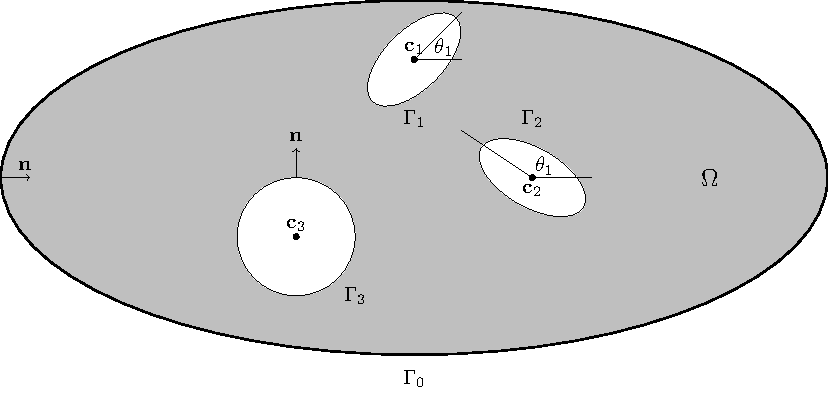
\includegraphics{figures/multiply_connected.pdf}}
\caption{A sketch of a bounded fluid domain $\Omega$.  $\gamma_1$ and
  $\gamma_2$ enclose rigid particles, while $\Gamma_1$ is a solid wall.
  If $\Omega$ is unbounded,  $\Gamma_0$  is not present.  The vector
  $\nn$ is the unit normal vector pointing out of the fluid
domain.\label{fig:geomSchematic}}
\end{figure}

%%%%%%%%%%%%%%%%%%%%%%%%%%%%%%%%%%%%%%%%%%%%%%%%%%%%%%%%%%%%%%%%%%%%%%%%%%%%%%%
\subsection{Governing Equations}\label{sec:governing}

We are interested in small particles and slow velocities which renders
the Reynolds number small ($\Re \ll 1$), and the fluid is governed by the
incompressible Stokes equations.  A Dirichlet boundary condition $\UU$
is imposed on the solid walls $\Gamma$, a no-slip boundary condition is
imposed on the rigid bodies $\gamma$, and the rigid bodies are assumed
to be force- and torque-free.  On each solid wall, there is a net force
and torque, $\FF^\Gamma_i$ and $L^\Gamma_i$, respectively, that depend
on the boundary condition.  A similar force, $\FF^\gamma_j$, and torque
$L^\gamma_j$ are defined for each rigid body $\gamma_j$, but these, for
the time being, are assumed to be 0.  Therefore, the governing equations
for $M_p$ particles suspended in a bounded $M_w$-connected domain is
\begin{equation}
  \label{eqn:modelEquations}
  \begin{aligned}
  \mu \Delta \uu = \grad p, &\hspace{20pt} \xx \in \Omega, \gap
    &&\mbox{\it conservation of momentum,}\\
  \grad \cdot \uu = 0, &\hspace{20pt} \xx \in \Omega, \gap
    &&\mbox{\it conservation of mass,} \\
  \uu = \UU, &\hspace{20pt} \xx \in \Gamma, \gap 
    &&\mbox{\it wall velocity,} \\
  \uu = \uu^\tau_j + \omega_j(\xx-\cc^\gamma_j)^\perp,&\hspace{20pt} 
    \xx \in \gamma, \gap &&\mbox{\it no-slip on the bodies,} \\
  \FF_j^\gamma = 0, &\hspace{20pt}j=1,\ldots,M_p, \gap 
    &&\mbox{\it force-free bodies,} \\
  L_j^\gamma = 0, &\hspace{20pt}j=1,\ldots,M_p, \gap 
    &&\mbox{\it torque-free bodies.}
  \end{aligned}
\end{equation}
Here, $\uu$ is the velocity, $p$ is the pressure, $\mu$ is the fluid
viscosity, $\uu^\tau_j$ and $\omega_j$ are the translational and
rotational velocities of rigid body $j$, respectively, and
$\FF_j^\gamma$ and $L_j^\gamma$ are the net force and torque of rigid
body $j$.  In the Stokes limit, the fluid viscosity sets
the time scale, and we assume it is one throughout the paper.  In the
case that the fluid domain is unbounded, the wall velocity equation is
replaced with the far-field condition
\begin{align*}
  \uu(\xx) = \uu_\infty(\xx), \quad |\xx| \rightarrow \infty.
\end{align*}
Upon solving for the translational and rotational velocities, the rigid
body centers and inclination angles $(\cc_j,\theta_j)$,
$j=1,\ldots,M_p$, satisfy
\begin{align}
  \frac{d\cc_j}{dt} = \uu^\tau_j, \qquad 
  \frac{d\theta}{dt} = \omega_j.
\label{eqn:centersAngles}
\end{align}
Equations~\eqref{eqn:modelEquations} and~\eqref{eqn:centersAngles} govern
the dynamics of the rigid body suspensions, and their numerical solution
is a focus of this paper.

We have assumed that the suspension only has hydrodynamic forces.
However, when rigid bodies are brought sufficiently close together,
numerical errors can cause the rigid bodies to unphysically intersect.
To avoid contact,  we will later introduce a contact force that
guarantees that numerical errors do not cause rigid bodies to come into
contact.  This idea is first described for vesicle suspensions by Lu et
al.~\cite{Lu2017} and we summarize the method in
Section~\ref{sec:repulsion}.  


%%%%%%%%%%%%%%%%%%%%%%%%%%%%%%%%%%%%%%%%%%%%%%%%%%%%%%%%%%%%%%%%%%%%%%%%%%%%%%%
\subsection{Boundary Integral Equation Representation}
There exist many numerical methods for
solving~\eqref{eqn:modelEquations} such as level set
methods~\cite{Dou2007}, immersed boundary methods~\cite{Mittal2005},
dissipative particle dynamics~\cite{Pivkin2010}, smoothed particle
hydrodynamics~\cite{Polfer2016}, and lattice Boltzmann
methods~\cite{Ladd1994a, Ladd1994b}. However, because the fluid
equations are linear, a boundary integral equation (BIE)
formulation~\cite{Pozrikidis1992} is possible.  BIEs have several
advantages including that only the interface has to be tracked, which
simplifies the representation of complex and moving geometries, and
high-order discretizations are straightforward.  We now reformulate
equation~\eqref{eqn:modelEquations} as a BIE.

We start by formulating the incompressible Stokes equations in the
absence of rigid bodies.  The {\em double-layer potential} is the
convolution of the stresslet with an arbitrary density
function~\cite{Ladyzhenskaya1963, Pozrikidis1992},
\begin{align}
  \label{eqn:dlp}
  \uu(\xx) = \DD[\eeta](\xx) = \frac{1}{\pi}\int_{\Gamma}
  \frac{\rr\cdot\nn}{\rho^2}\frac{\rr \otimes \rr}{\rho^2}
  \eeta(\yy)~\text{d}s_{\yy}, \quad \xx \in \Omega,
\end{align}
where $\rr = \xx - \yy$, $\rho=|\rr|$, and $\eeta$ is an unknown density
function defined on $\bd\Omega$.  The double-layer
potential~\eqref{eqn:dlp} satisfies the incompressible Stokes equations,
and the Dirichlet boundary condition $\UU$ is also satisfied if
$\eeta$ satisfies~\cite{Pozrikidis1992}
\begin{align}
  -\frac{1}{2} \eeta(\xx_0) + \DD[\eeta](\xx_0) = \UU(\xx_0), 
    \quad \xx_0 \in \Gamma.
  \label{eqn:secondKindBIE}
\end{align}
The double-layer potential cannot represent rigid body motions that
satisfy the incompressible Stokes equations.  Following Power and
Miranda~\cite{Power1987, Power1993}, this is resolved by introducing
point forces and torques due to each interior component of the geometry
$\Gamma_j$, and the strengths of these forces and torques are related to
the density function $\eeta$.  The velocity fields due to a point force
(Stokeslet) and a point torque (rotlet), both centered at $\cc$, are
\begin{align*}
  \mathbf{S}(\xx,\cc) = \frac{1}{4\pi}\left(-\log\rho\mathbf{I} + 
  \frac{\rr \otimes \rr}{\rho^2}\right), \quad \text{and} \quad
  \mathbf{R}(\xx,\cc) = \frac{\rr^\perp}{4\pi\rho^2},
\end{align*}
where $\rr = \xx - \cc$ and $\rho = |\rr|$.  Then, the second-kind
integral equation~\eqref{eqn:secondKindBIE} is replaced with the
completed second-kind BIE
\begin{equation}
  \label{eqn:completed_DLP}
  \begin{aligned}
  -\frac{1}{2}\eeta(\xx_0) + \DD[\eeta](\xx_0) + 
    \sum_{j=1}^{M_w} \left(\mathbf{S}(\xx,\cc^\Gamma_j)\FF^\Gamma_j + 
      \mathbf{R}(\xx,\cc^\Gamma_j)L^\Gamma_j\right) &= \UU(\xx_0),
      \quad &&\xx_0 \in \Gamma, \\
  \int_{\Gamma_j} \eeta~\text{d}s &= \FF^\Gamma_j, 
      &&j=1,\ldots,M_w, \\
  \int_{\Gamma_j} \eeta\cdot (\xx - \cc^\Gamma_j)^\perp~\text{d}s &=   
      L^\Gamma_j, &&j=1,\ldots,M_w.
\end{aligned}
\end{equation}

We now introduce a suspension of rigid bodies $\gamma_j$,
$j=1,\ldots,M_p$.  The double-layer potential now includes contributions
from both the solid walls and rigid bodies.  Imposing the no-slip
boundary condition on the rigid bodies, a BIE formulation for a
suspension of rigid bodies governed by
equation~\eqref{eqn:modelEquations} is
\begin{subequations}
  \label{eqn:BIEformulation}
  \begin{align}
    \UU(\xx) &= -\frac{1}{2}\eeta(\xx) + \DD[\eeta](\xx) +
    \sum_{j=1}^{M_w} \left(\mathbf{S}(\xx,\cc^\Gamma_j)\FF^\Gamma_j + 
      \mathbf{R}(\xx,\cc^\Gamma_j)L^\Gamma_j\right)  \nonumber \\
&\hspace{96pt}+\sum_{j=1}^{M_p} \left(\mathbf{S}(\xx,\cc^\gamma_j)\FF^\gamma_j +
\mathbf{R}(\xx,\cc^\gamma_j)L^\gamma_j\right),
    \quad \xx \in \Gamma, \label{eqn:BIEformulation1} \\
  \uu^\tau_j + \omega_j(\xx - \cc_j^\gamma)^\perp &=
    -\frac{1}{2}\eeta(\xx) + \DD[\eeta](\xx) + 
    \sum_{j=1}^{M_w} \left(\mathbf{S}(\xx,\cc^\Gamma_j)\FF^\Gamma_j + 
      \mathbf{R}(\xx,\cc^\Gamma_j)L^\Gamma_j\right) \nonumber \\
&\hspace{96pt}+\sum_{j=1}^{M_p} \left(\mathbf{S}(\xx,\cc^\gamma_j)\FF^\gamma_j +
\mathbf{R}(\xx,\cc^\gamma_j)L^\gamma_j\right),
    \quad \xx \in \gamma, \label{eqn:BIEformulation2} \\
  \int_{\Gamma_j} \eeta~\text{d}s &= \FF^\Gamma_j, \quad
  \int_{\Gamma_j} \eeta\cdot (\xx - \cc^\Gamma_j)^\perp~\text{d}s =
  L^\Gamma_j, \quad j=1,\ldots,M_w, \label{eqn:BIEformulation3} \\
  \int_{\gamma_j} \eeta~\text{d}s &= \FF^\gamma_j, \quad
  \int_{\gamma_j} \eeta\cdot (\xx - \cc^\gamma_j)^\perp~\text{d}s =
  L^\gamma_j,\quad j=1,\ldots,M_p, \label{eqn:BIEformulation4} \\
  \FF^\gamma_j &= 0, \quad L^\gamma_j = 0,\quad j=1,\ldots,M_p.
  \label{eqn:BIEformulation5}
\end{align}
\end{subequations}
Again, the methodology of Power and Miranda relates the strength of the
Stokeslets and rotlets of each rigid body to its density function.  The
BIE formulation~\eqref{eqn:BIEformulation} of the governing
equations~\eqref{eqn:modelEquations} consists of eight equations for
eight unknowns: the density function, net force, and net torque on the
solid walls and rigid bodies, and the translational and rotational
velocities.

While~\eqref{eqn:BIEformulation1} and~\eqref{eqn:BIEformulation2} are
both numerically desirable second-kind Fredholm integral equations
equations, equation~\eqref{eqn:BIEformulation1} has a rank one null
space because of the flux-free condition of the boundary data
$\UU$~\cite{Ladyzhenskaya1963}.  Following Power~\cite{Power1993}, this
null space is removed by adding the term 
\begin{align}
\label{eqn:N0_modification} 
  \mathcal{N}_0[\eeta](\xx) = \int_{\Gamma_0} 
    \nn(\xx)\otimes\nn(\yy)~\text{d}s(\yy)
\end{align}
to~\eqref{eqn:BIEformulation1}, but only for points $\xx \in \Gamma_0$.
If $\Omega$ is unbounded, equation~\eqref{eqn:BIEformulation} has no
null space, and the only modification is that
equation~\eqref{eqn:BIEformulation1} is removed, and the background
velocity $\uu_\infty(\xx)$ is added to the right hand side of
equation~\eqref{eqn:BIEformulation2}.

Finally, to understand the rheological and statistical properties of
suspensions of rigid bodies, it is necessary to compute the pressure,
stress, and energy dissipation.  Formulas for these quantities are layer
potentials involving the density function $\eeta$~\cite{Power1993}.  A
numerical method for computing these layer potentials is described
in~\ref{sec:spatial}.


%%%%%%%%%%%%%%%%%%%%%%%%%%%%%%%%%%%%%%%%%%%%%%%%%%%%%%%%%%%%%%%%%%%%%%%%%%%%%%%
\subsection{A Contact-Based Repulsion Force}
\label{sec:repulsion}
Exact solutions of the Stokes equations prohibit contact between force-
and torque-free bodies in finite time.  Therefore, any contact between
rigid bodies is caused by numerical errors.  The two main sources of
error are the quadrature error and time stepping error.  We address the
quadrature error using a combination of upsampling and interpolation,
and details of the method are described in~\cite{Quaife2014}.  Time
stepping methods have recently received a lot of attention, and some
recent works address stiffness~\cite{Quaife2014} and adaptive time
stepping~\cite{Kropinski1999, Quaife2015, Sorgentone2018}.  We describe
time stepping methods in Section~\ref{sec:temporal}.

We adopt the method of using artificial forces to avoid contact, and
there are many choices for the force. One possibility is a Morse or
Lennard-Jones potential that grows as a high order polynomial as two
bodies approach~\cite{Flormann2017, Liu2006}. This has been shown to
work for dense suspensions, but the resulting dynamics for the rigid
body dynamics become very stiff as the separation between bodies
decreases.  Spring models~\cite{Tsubota2006, Kabacogulu2017} have also
been used to generate artificial repulsion forces, but these models also
introduce stiffness. A further disadvantage of many contact algorithms
is that they do not guarantee that particles remain contact-free.

We apply a modification of the contact-aware method of Lu et
al.~\cite{Lu2017} that explicitly requires that particles remain
contact-free. We only summarize the method, but an in-depth description
is in the original work~\cite{Lu2017}.  To apply a Lagrange multiplier
method, the governing equations~\eqref{eqn:modelEquations} are written
as a constrained optimization problem by using the variational form of
the Stokes equations
\begin{align}
  \min \int_{\Omega} \nabla\uu:\nabla\uu~\text{d}\Omega,
  \quad\text{ such that }\quad \nabla\cdot\uu = 0, 
  \quad \xx \in \Omega.
  \label{eqn:stokesEL}
\end{align} 
After taking a time step, all pairs of bodies whose separation falls
below a minimum separation distance, which includes those that have
collided, are flagged.  Then, the space-time interference volume (STIV),
defined as the volume in space-time distance swept out by the trajectory
of two bodies, is computed.  The STIV offers a metric to quantify the
amount of collision that occurs between two bodies~\cite{Lu2017,
Harmon2011}.  Next, equation~\eqref{eqn:stokesEL} is supplemented with
an additional constraint that the STIV is positive (no contact).  By
computing the STIV, rather than simply the overlap at the new time step,
time steps that result in rigid bodies passing through each other are
detected and resolved.  Details for solving~\eqref{eqn:stokesEL} with
the STIV inequality constraint are given in Section~\ref{sec:contact}.

%%%%%%%%%%%%%%%%%%%%%%%%%%%%%%%%%%%%%%%%%%%%%%%%%%%%%%%%%%%%%%%%%%%%%%%%%
%\subsection{Computing the Pressure and Stress}
%To understand the rheological and statistical properties of suspensions
%of rigid bodies, it is necessary to compute the pressure, stress, and
%energy dissipation.  This expressions are standard~\cite{Power1993}, but
%we summarize them for completeness.  A numerical method for computing
%the pressure, stress, and energy dissipation is described in
%Section~\ref{sec:spatial}.
%
%The pressure of the two-dimensional double-layer potential
%is~\cite{Power1993}
%\begin{align*}
%  p(\xx) = \frac{1}{\pi}\int_{\partial\Omega}\frac{1}{\rho^2}\left(
%\mathbf{I} - 2\frac{\rr \otimes \rr}{\rho^2}\right)\nn\cdot\eeta~\text{d}s,
%\qquad\xx\in\Omega.
%\end{align*}
%The pressure of the Stokeslet and rotlet contributions are easily
%computed, and the pressure of the completed double-layer
%potential~\eqref{eqn:completed_DLP} is
%\begin{align}
%  \label{eqn:pressure} 
%  p(\xx) = \frac{1}{\pi}\int_{\partial\Omega}\frac{1}{\rho^2}\left(
%    \mathbf{I} - 2\frac{\rr \otimes \rr}{\rho^2}\right)\nn\cdot\eeta~\text{d}s +
%  \sum_{i=1}^{M_w}
%  \frac{\FF_i^\Gamma\cdot(\xx-\cc_i^\Gamma)}{2\pi|\xx-\cc_i^{\Gamma}|^2}
%  + \sum_{i=1}^{M_p}
%    \frac{\FF_i^\gamma\cdot(\xx-\cc_i^\gamma)}{2\pi|\xx-\cc_i^\gamma|^2}.
%\end{align}
%
%Starting with the pressure~\eqref{eqn:pressure}, we compute the stress
%tensor
%\begin{align*} 
%\ssigma = -p \mathbf{I} + \left(\nabla \uu + (\nabla\uu)^\intercal\right), \qquad
%\xx\in\Omega.
%\end{align*}
%We decompose the stress into contributions from the double-layer
%potential, Stokeslets, and rotlets
%\begin{align}
%  \label{eqn:stress}
%  \ssigma = \ssigma_{\eeta} + \ssigma_{S} + \ssigma_{R},
%\end{align}
%where
%\begin{align*}
%  \ssigma_{\eeta}(\xx) &= \frac{1}{\pi}\int_{\partial\Omega}\left( 
%    \frac{\nn\cdot\eeta}{\rho^2}\mathbf{I} 
%    -8\frac{(\rr\cdot\nn)(\rr\cdot\eeta)(\rr\otimes\rr)}{\rho^6} 
%    +\frac{(\rr\cdot\nn)(\rr\otimes\eeta + \eeta\otimes\rr)}{\rho^4} 
%+ \frac{(\rr\cdot\eeta)(\rr\otimes\nn +
%\nn\otimes\rr)}{\rho^4}\right)\text{d}s,\\
%  \ssigma_S(\xx) &= -\sum_{i=1}^{M_w} 
%    \frac{\FF_i^\Gamma\cdot(\xx - \cc_i^\Gamma)}{\pi|\xx-\cc_i^\Gamma|^2}
%        (\xx - \cc_i^\Gamma)\otimes(\xx - \cc_i^\Gamma)  -
%    \sum_{i=1}^{M_p}
%    \frac{\FF_i^\gamma\cdot(\xx - \cc_i^\gamma)}{\pi|\xx-\cc_i^\gamma|^2}
%        (\xx-\cc_i^\gamma )\otimes(\xx-\cc_i^\gamma),\\
%\ssigma_R(\xx) &= -\sum_{i=1}^{M_w} \frac{L_i^\Gamma}{2\pi|\xx-\cc_i^\Gamma|^2}
%((\xx-\cc_i^\Gamma)\otimes(\xx-\cc_i^\Gamma)^\perp +
%    (\xx-\cc_i^\gamma)^\perp\otimes(\xx-\cc_i^\gamma))  \\
%\qquad&-\sum_{i=1}^{M_p}
%\frac{L_i^\gamma}{2\pi|\xx-\cc_i^\gamma|^2}
%    ((\xx-\cc_i^\gamma )\otimes(\xx-\cc_i^\gamma)^\perp + 
%    (\xx-\cc_i^\gamma)^\perp\otimes(\xx-\cc_i^\gamma)).
%\end{align*}
%
%These expressions hold inside $\Omega$. On the boundary there is a jump
%in the pressure and stress, as reported in~\cite{Quaife2014}.  These
%boundary terms are required for our near-singular integration scheme
%described in Section~\ref{sec:spatial}.  Finally, using the divergence
%theorem, the volumed average stresses can be expressed in terms of
%boundary integrals (see Section 2.5 in
%Pozrikidis~\cite{Pozrikidis1992}). 
		
%%%%%%%%%%%%%%%%%%%%%%%%%%%%%%%%%%%%%%%%%%%%%%%%%%%%%%%%%%%%%%%%%%%%%%%
\section{Numerical Methods}\label{s:method}
We are ultimately interested in studying statistical and rheological
properties of the fiber suspensions.  Therefore, we develop stable
numerical methods that solve the governing
equations~\eqref{eqn:modelEquations} for long time horizons.  To achieve
high-order accuracy, the spatial grid is resolved with spectral accuracy
(Section~\ref{sec:spatial}), and stability is achieved by using implicit
interactions in the time integrator and adaptive time stepping
(Section~\ref{sec:temporal}).  We are much more concerned with stability
than accuracy, so we use low-order but stable time stepping schemes.
Each time step requires solving a block diagonal preconditioned dense
linear system that is solved with GMRES and accelerated with the fast
multipole method~\cite{Greenbaum1992} (Section~\ref{sec:fast}).  We also
discuss a numerical methods for the collision algorithm
(Section~\ref{sec:contact}), and for computing the pressure and stress
(Section~\ref{sec:pressure_stress}).


%%%%%%%%%%%%%%%%%%%%%%%%%%%%%%%%%%%%%%%%%%%%%%%%%%%%%%%%%%%%%%%%%%%%%%%
\subsection{Spatial Discretization}\label{sec:spatial}
Let $\xx_j(\alpha)$, $\alpha \in [0,2\pi)$, be a parameterization of a
rigid body $\gamma_j$.  We use a collocation method that requires
the discretization points $\xx_k$ for $k=1,\ldots,N_p$.  Spectral
accuracy is achieved by representing functions defined on $\gamma_j$ as
a Fourier series
\begin{align}
  f(\alpha) = f(\xx_j(\alpha)) = 
    \sum_{k = 0}^{N_p-1} \hat{f}_k e^{ik\alpha}.
\end{align}
The rigid walls are identically discretized at $N_w$ points and
functions defined on the rigid walls are also represented as a Fourier
series.  We use the FFT to compute the Fourier coefficients, and all
derivatives are computed with spectral accuracy by differentiating in
Fourier space.

With collocation points defined on the solid bodies and rigid walls, we
now discretize the layer potentials.  We use a Nystr\"om method by
approximating the double-layer potentials with the trapezoid rule.
Equation~\eqref{eqn:BIEformulation} is discretized as
\begin{equation*}
  \begin{aligned}
  \UU(\xx_i) = -\frac{1}{2}\eeta(\xx_i) + 
  \sum_{k=1}^{N} K(\xx_i,\xx_k) \eeta(\xx_k) \Delta s_k
    + \sum_{j=1}^{M_p} \left(\mathbf{S}(\xx_i,\cc^\gamma_j)\FF_j +
    \mathbf{R}(\xx_i,\cc_j)L_j\right) 
    + \sum_{j=1}^{M_w} \left(\mathbf{S}(\xx_i,\cc^\Gamma_j)\FF_j +
    \mathbf{R}(\xx_i,\cc^\Gamma_j)L_j\right),
  \end{aligned}
\end{equation*}
for $\xx_i \in \Gamma$, and
\begin{equation*}
  \begin{aligned}
\uu^\tau_j + \omega_j(\xx_i - \cc^\gamma_j)^\perp =
-\frac{1}{2}\eeta(\xx_i) +
\sum_{k=1}^{N} K(\xx_i,\xx_k) \eeta(\xx_k) \Delta s_k
    &+ \sum_{j=1}^{M_p} \left(\mathbf{S}(\xx_i,\cc^\gamma_j)\FF_j +
    \mathbf{R}(\xx_i,\cc_j)L_j\right) 
    + \sum_{j=1}^{M_w} \left(\mathbf{S}(\xx_i,\cc^\Gamma_j)\FF_j +
    \mathbf{R}(\xx_i,\cc^\Gamma_j)L_j\right),
  \end{aligned}
\end{equation*}
for $\xx_i \in \gamma_j$, where $N = M_w N_w + M_p N_p$ is the total
number of discretization points and
\begin{align*}
  K(\xx,\yy) = \frac{1}{\pi} \frac{\rr \cdot \nn}{\rho^2} 
               \frac{\rr \otimes \rr}{\rho^2}
\end{align*}
is the kernel of the double-layer potential.  The diagonal entries of
$K$ are replaced with the limiting value
\begin{align*}
  \lim_{\substack{\yy \rightarrow \xx \\ \yy \in \bd\Omega}} 
    K(\xx,\yy) = \frac{\kappa}{2\pi}\tt\otimes\tt,
    \quad \xx \in \bd\Omega,
\end{align*}
where $\kappa(\xx)$ is the curvature and $\tt(\xx)$ is the tangent
vector of $\bd\Omega$ at $\xx$.

Since the kernel $K(\xx,\yy)$ is smooth, the trapezoid rule guarantees
spectral accuracy~\cite{Trefethan2014}.  However, at a fixed resolution
$N$, the error grows when a target point and a source point on different
bodies approach one another.  The error is caused by a nearly-singular
integrand with large derivatives.  To resolve this issue, an algorithm
for near-singular integration method must be employed.  We use the
interpolation scheme outlined in~\cite{Quaife2014} that is based off of
the algorithm first outlined in~\cite{Ying2006}.
  
After discretizing~\eqref{eqn:BIEformulation} with a Nystr\"om method,
the result is a dense linear system for the density function, rotlets
and Stokeslets, and the translational and rotational velocities of each
body.  We chose a double-layer potential formulation so that the linear
system can be solved with a mesh-independent number of GMRES
iterations~\cite{Campbell1996}.  Therefore, the algorithmic cost is
dominated by the cost of a matrix-vector multiplication, and the number
of required geometry-dependent GMRES iterations.  Algorithms for
controlling these costs are discussed in Section~\ref{sec:fast}.

%%%%%%%%%%%%%%%%%%%%%%%%%%%%%%%%%%%%%%%%%%%%%%%%%%%%%%%%%%%%%%%%%%%%%%%%
\subsection{Contact Resolution}
\label{sec:contact}
The contact resolution method starts by advancing the force- and
torque-free bodies from time $t$ to $t + \Delta t$ with
equation~\eqref{eqn:centersAngles}.  Then, equation~\eqref{eqn:stokesEL}
needs to be solved with the inequality constraint that the STIV is
greater than zero.  The definition of the STIV includes a parameter that
guarantees that not only do bodies not intersect, but they maintain
minimum separation distance. Following~\cite{Lu2017}, each pair of
colliding bodies is given a single Lagrange multiplier that is used to
satisfy the non-negative STIV inequality constraint (a negative STIV
indicates contact).  The resulting equations are the incompressible
Stokes equations with body forces and torques that depend on the
gradient of the STIV, and the inequality constraint that the STIV is
less than or equal to zero.  Therefore, the governing equations are
similar to~\eqref{eqn:BIEformulation}, except that the force- and
torque-free conditions have been changed.

The resulting equation is a non-linear complementary problem (NCP). To
solve the NCP, the problem is linearized as a sequence of linear
complementary problems (LCPs) that are solved until the STIV is less
than or equal to zero.  For small minimum separation distances, it is
possible that the LCP converges very slowly, or not at all, to the
solution of the NCP.  In Section~\ref{sec:temporal}, we describe two
methods to avoid this slow convergence.

If only two bodies are in contact, Newton's third law is guaranteed by
the symmetry of the STIV.  However, if more than two bodies are in
contact, then the forces returned by the STIV are not guaranteed to sum
to zero.  We improve the validity of the method by always requiring that
the total force added to the system is zero, meaning
\begin{align*}
  \sum_{j=1}^{M_p} \FF^\gamma_j = \mathbf{0}. 
\end{align*}
This could be accomplished by introducing additional Lagrange
multipliers, and the result would be a modification to our governing
equations~\eqref{eqn:BIEformulation}.  As a simpler alternative, we
group all bodies that are in contact into distinct clusters.  For each
cluster, and at each NCP iteration, the body that is in contact with the
most other bodies (to break ties, we use the body with the largest
repulsion force in magnitude) is given a net force that balances all
other bodies in the cluster. Whenever a force on a body is scaled the
torque on that body is scaled by the same amount.

%%%%%%%%%%%%%%%%%%%%%%%%%%%%%%%%%%%%%%%%%%%%%%%%%%%%%%%%%%%%%%%%%%%%%%%
\subsection{Time Stepping Methods}
\label{sec:temporal}
Since we consider rigid body suspensions, we only track the centers
$\cc_i^\gamma$ and orientations $\theta_i$ of each rigid body
$\gamma_i$.  Substituting the no-slip boundary condition into
equation~\eqref{eqn:BIEformulation}, the center and orientation of a
suspension of rigid bodies satisfies
\begin{align*}
  \frac{d\cc_i^\gamma}{dt} + \frac{d\theta_i}{dt}
    (\xx - \cc_i^\gamma)^\perp &=
    -\frac{1}{2}\eeta(\xx) + \DD[\eeta](\xx) + 
    \sum_{j=1}^{M_w} \left(\mathbf{S}(\xx,\cc^\Gamma_j)\FF^\Gamma_j + 
      \mathbf{R}(\xx,\cc^\Gamma_j)L^\Gamma_j\right) 
    +\sum_{j=1}^{M_p} \left(\mathbf{S}(\xx,\cc^\gamma_j)\FF^\gamma_j +
      \mathbf{R}(\xx,\cc^\gamma_j)L^\gamma_j\right).
\end{align*}
After discretizing this equation with forward Euler, the result is an
equation for the new center, inclination angle, and density function
(including the rotlets and Stokeslets) in terms of the old centers,
inclination angles, net forces, and net torques.  An equivalent
formulation is to freeze the rigid bodies at the current time step,
solve~\eqref{eqn:BIEformulation} for $\uu^\tau_k$, $\omega_k$, and
$\eeta$, and then update the position and angle of each body by
discretizing the differential equations
\begin{align*}
  \frac{\text{d}}{\text{d}t}\cc_k &= \uu^\tau_k,  
    \quad \cc_k(t^N) = \cc_k^N, \\
  \frac{\text{d}}{\text{d}t}\theta_k &= \omega_k,
    \quad \theta_k(t^N) = \theta_k^N,
\end{align*}
with the first-order explicit Euler method
\begin{align*}
  \cc_k^{N+1} &= \cc_k^N + \Delta t \left(\uu_k^\tau\right)^N, \\
  \theta_k^{N+1} &= \theta_k^N + \Delta t \left(\omega_k\right)^N.
\end{align*}
A low cost first-order time stepper is justified since we are interested
in statistical, rheological, and bulk quantities rather than the
individual trajectories of the rigid bodies.  If high-order accuracy is
desired, a Runge-Kutta or deferred correction method~\cite{Quaife2015,
qua-bir2016} can be applied.

The main factors that determine the stiffness of the system are the
minimum separation distance and the discretization of the double-layer
potential $\DD[\eeta](\xx)$.  The leading source of stiffness is the
velocity field caused by the body itself. This stiffness can be
controlled by discretizing the double-layer potential as
\begin{align}
  \DD[\eeta](\xx) \approx \DD^{N}_{i,i}\left[\eeta_i^{N+1}\right](\xx) + 
    \sum_{k \neq i} \DD^{N}_{i,k}\left[\eeta_k^{N}\right](\xx),
    \quad \xx \in \gamma_i,
  \label{eqn:BlockImplicit}
\end{align}
where $\DD_{i,k}^N$ is the double-layer potential due to body $\gamma_k$
evaluated on $\gamma_i$, with both these bodies discretized at time $N$.
This time stepping method has the advantage that only the density
function due to intra-particle interactions are treated implicitly,
while the density function computed at the previous time step is used to
approximate the inter-particle interactions.  The result is a
block-diagonal system for the new density function.  This time stepping
method is the focus of the work of Lu et al.~\cite{Lu2017}, and since
only the intra-particle interactions are discretized implicitly, they
call the method a {\em locally implicit} discretization.  The next
source of stiffness is caused by nearly-touching bodies, which can be
controlled by maintaining a sufficiently large minimum separation
distance~\cite{Lu2017}.  Alternatively, to allow for small minimum
separation distances, we discretize the interaction between
nearly-touching bodies implicitly as
\begin{align}
  \DD[\eeta](\xx) \approx \DD^{N}_{i,i}\left[\eeta_i^{N+1}\right](\xx) + 
    \sum_{k \neq i} \DD^{N}_{i,k}\left[\eeta_k^{N+1}\right](\xx),
    \quad \xx \in \gamma_i.
  \label{eqn:SemiImplicit}
\end{align}
Rather than using the density function from the previous time step, this
method solves for the density function corresponding to the current
rigid body suspension.  Since all the bodies are coupled, the method is
called a {\em globally implicit} discretization.  In
Section~\ref{s:results}, we demonstrate that this new time stepping
method is able to take larger stable time step sizes for dense
suspensions of rigid bodies.  In addition, when the contact algorithm is
required, the globally implicit discretization~\eqref{eqn:SemiImplicit}
requires fewer LCP iterations to converge to a solution of the NCP when
compared to the locally implicit
discretization~\eqref{eqn:BlockImplicit}.

Finally, since the dynamics of the suspension can develop complex
features, the time step size should be adjusted accordingly.  If the
error can be efficiently estimated at each time step, the time step size
can be adjusted according to this estimate.  However, such estimates
require multiple numerical solutions or a physical quantity, such as the
fluid mass in a control region, that is easy to compute and conserved by
the governing equations.  Forming multiple numerical solutions is too
expensive, and our simulations do not have an conserved quantity that we
can easily compute.  Therefore, rather than trying to control the error
at each time step, we use a heuristic adaptive time stepping method.
When the LCP solver requires many iterations to solve the NCP, this
indicates that the time step size should be reduced.  Conversely, if the
LCP solver converges quickly to the solution of the NCP, then a larger
time step size can be taken.  Therefore, if each LCP iteration is not
converging to a contact-free configuration sufficiently fast, we abort
the time step and restart with the time step size $\Delta t/2$.
Conversely, if the LCP iteration converges quickly, then, at the next
time step, we increase $\Delta t$ to $1.5\Delta t$. This strategy can
not be used to guarantee a user-specified error bound.  However, it does
appropriately adjust the time step size according to the dynamics, and
the result is that simulations are able to reach their time horizon
without taking wastefully uniform small time step size.

%%%%%%%%%%%%%%%%%%%%%%%%%%%%%%%%%%%%%%%%%%%%%%%%%%%%%%%%%%%%%%%%%%%%%%%
\subsection{Fast Summation and Preconditioning}
\label{sec:fast}
A discretization of the locally implicit time
stepper~\eqref{eqn:BlockImplicit} results in a block-diagonal linear
system, where each block is a dense $N_p \times N_p$ or $N_w \times N_w$
matrix.  In contrast, a discretization of the globally implicit time
stepper~\eqref{eqn:SemiImplicit} results in a dense $N \times N$ linear
system.  Therefore, considering only the rigid body contributions, the
cost of a single matrix-vector multiplication is $\mathcal{O}(M_p
N_p^2)$ for~\eqref{eqn:BlockImplicit} and $\mathcal{O}(M_p^2 N_p^2)$
for~\eqref{eqn:SemiImplicit}.  We reduce the cost of matrix-vector
multiplication by using the fast multipole method.  This reduces the
cost of a single matrix-vector multiplication for both the locally
implicit and globally implicit time stepping methods to $\mathcal{O}(N)$
operations.

Reducing the cost of matrix-vector multiplication greatly reduces the
computational effort.  However, even though we are solving a
well-conditioned second-kind integral equation, for dense suspensions,
the number of GMRES iterations can be prohibitively large.  Therefore,
we apply a block-diagonal preconditioner where each block is precomputed
and factorized.  The identical preconditioner has been used for
two-dimensional vesicle suspensions~\cite{Quaife2014}.  Without
preconditioning, the dense suspension in Section~\ref{sec:taylor_green}
requires, on average, 100 GMRES iterations per time step. However, by
applying the block-diagonal preconditioner, the average number of GMRES
iterations is reduced to 50 per time step.  Moreover, since we are
considering rigid body suspensions, the block-diagonal preconditioner of
a new configuration can be formed by multiplying the previous
preconditioner with the rotation matrix corresponding to the rotation
velocity $\omega$.  Therefore, the preconditioner only needs to be
computed and factorized once for the entire simulation, and it is
updated at each time step with a negligible computational cost.


%%%%%%%%%%%%%%%%%%%%%%%%%%%%%%%%%%%%%%%%%%%%%%%%%%%%%%%%%%%%%%%%%%%%%%%
\subsection{Computing the Pressure and Stress}
\label{sec:pressure_stress}
Computing the layer potentials for the pressure and stress is more
challenging than evaluating the velocity double-layer potential.  The
challenge stems from a singularity that scales as $\mathcal{O}(|\xx -
\yy|^{-2})$ as a target point approaches a source point.  The pressure
and stress are computed with spectral accuracy by using a combination of
singularity subtraction and odd-even integration~\cite{sid-isr1988}.
Near-singular integration is still required, and our interpolation-based
method requires limiting values of the layer potentials as $\xx
\rightarrow \bd\Omega$.  The limiting values and tests of the
near-singular integration scheme are reported in~\cite{Quaife2014}.
Finally, using the divergence theorem, the volume average stresses are
expressed in terms of boundary integrals~\cite{Pozrikidis1992} (see
Section 2.5).

%%%%%%%%%%%%%%%%%%%%%%%%%%%%%%%%%%%%%%%%%%%%%%%%%%%%%%%%%%%%%%%%%%%%%%%
\section{Results}\label{s:results}
We use our new time stepping method to simulate bounded and unbounded
suspensions of two-dimensional rigid bodies in a viscous fluid.  The
main parameters are the minimum separation distance $\delta$, the number
of discretization points of each body, $N_p$, and each solid wall,
$N_w$, and the initial time step size $\Delta t$. We perform temporal
convergence studies and investigate the effect of the STIV algorithm on
the reversibility of the flow.  To further demonstrate the consequence
of STIV, we include plots of pathlines that cross whenever the collision
detection algorithm is applied.  The particular experiments we perform
are now summarized.
\begin{itemize}
  \item {\bf Shear Flow}: We consider the standard problem of two
  identical rigid circles in the shear flow $\uu = (y,0)$ with one body
  placed to the left and slightly above the other body.  We report
  similar results to those presented in~\cite{Lu2017}, but the globally
  implicit time stepping method allows for smaller initial displacements
  and minimum separation distances.  The contact algorithm breaks the
  reversibility of the flow, and this effect is illustrated and
  quantified.

  \item {\bf Taylor-Green Flow}: We simulate a concentrated suspension
  of 48 rigid ellipses in an unbounded Taylor-Green flow. At the
  prescribed separation distance, our new time stepping method is able
  to stably reach the time horizon, while the locally semi-implicit time
  integrator proposed by Lu et al.~\cite{Lu2017} results in the STIV
  contact algorithm not converging, even with $\Delta t = 10^{-8}$.

  \item {\bf Porous Monolayer Injection}: We consider a suspension of
  confined rigid circular bodies motivated by an experiment by MacMinn
  et al.~\cite{MacMinn2015}.  The geometry is an annulus with an inflow
  at the inner boundary and an outflow at the outer boundary.  We again
  examine the effect STIV on the reversibility of the flow, and compute
  the shear strain rate and make qualitative comparisons to results for
  deformable bodies~\cite{MacMinn2015}.

  \item {\bf Taylor-Couette Flow}: With the ability to do concentrated
  suspensions without imposing a large non-physical minimum separation
  distance, we simulate rigid bodies of varying aspect ratios inside a
  Taylor-Couette device.  We examine the effect of the rigid body shape
  and concentration on the effective viscosity and the alignment angles.
\end{itemize}



%%%%%%%%%%%%%%%%%%%%%%%%%%%%%%%%%%%%%%%%%%%%%%%%%%%%%%%%%%%%%%%%%%%%%%%
\subsection{Shear Flow}
\label{sec:shear}
We consider two rigid circular bodies in the shear flow ${\uu}(\xx) =
(y,0)$.  One body is centered at the origin, while the other body is
placed to the left and slightly above the body at the origin.  With this
initial condition, the particles come together, interact, and then
separate.  Both bodies are discretized with $N=32$ points and the arc
length spacing is $h = 2\pi/32 \approx 0.196$.  This experiment was also
performed by Lu et al.~\cite{Lu2017}, and we compare the locally
implicit and globally implicit time stepping methods.  We start by
considering the time step size $\Delta t = 0.4$ and minimum separation
distance $\delta = 0$ (no contact algorithm).  Our new globally implicit
method successfully reaches the time horizon without requiring a
repulsion force.  However, with the same $\Delta t$, locally implicit
time stepping results in a collision between the bodies, so the
collision algorithm is required to reach the time horizon.
Alternatively, the time step size can be reduced, but, as we will see,
for sufficiently dense suspensions, even an impractical small time step
size results in collisions.  

In Figure~\ref{fig:shear_experiment}, we investigate the effect of the
minimum separation distance on the position of the rigid bodies.  The
top plot shows the trajectory of the left body as it approaches,
interacts, and finally separates from the body centered at the origin.
The bottom left plot shows the trajectory of the particle when the
contact algorithm is applied with varying levels of separation.  Notice
that the trajectories are identical until near $x=0$ when the particle
separation first falls below the minimum separation distance.  Finally,
in the bottom right plot, the final vertical displacement body initially
on the left is plotted.  These simulations have also been performed with
the locally implicit time stepping method~\cite{Lu2017}, and the general
trend of the trajectories are similar.
\begin{figure}[t]
  \centerline{
  \includegraphics{figures/shear_setup1.pdf}}
  \centerline{
    \begin{tabular}{c c}
      \includegraphics{figures/shear_displacement1.pdf} &
      \includegraphics{figures/separation_displacement1.pdf}
    \end{tabular}
  }
\caption{\label{fig:shear_experiment} Shear experiment. Top: The initial
setup and trajectory of the left body.   Bottom left: The left body's
trajectory for varying minimum separation distances.  Notice how
the trajectories are identical until shortly before $x=0$ when the
contact algorithm is first applied.  Bottom right: The final vertical
displacement of the left particle for varying minimum separation
distances.}
\end{figure}

We next investigate the effect of the collision algorithm and time step
size on the reversibility of the flow. We reverse the shear direction at
$t=10$ and measure the error between the body's center at $t=0$ and
$t=20$.  We expect an error that is the sum of a first-order error
caused by time stepping, a fixed constant caused by the minimum
separation distance, and the spatial error which is negligible for the
time step sizes we consider.  The results for various values of $\delta$
and $\Delta t$ are reported in Table~\ref{tab:reverse}. The contact
algorithm is not required when $\delta=0$ and when $\delta=h$, and we
observe the expected first-order convergence.  However, when $\delta
\geq 2h$, the bodies are deflected onto contact-free pathlines when
their proximity reaches the minimum separation distance.  After the flow
is reversed, the bodies again pass one another, but they are now on
contact-free pathlines, so the initial deflection is not reversed.
Therefore, for these larger values of $\delta$, there is a decrease in
the error when the error is dominated by the time step size, but as
$\Delta t$ decreases, the error is dominated by the contact algorithm,
and the resulting error plateaus.

\begin{table}[t]
\caption{A study of time reversibility of the shear flow example. At
  $t=10$, the flow direction is reversed and we calculate the relative
  error in the initial and final positions. When the collision
  constraint is active and force is needed to keep the bodies apart the
  error in the reversibility is dominated by the contact
algorithm.\label{tab:reverse}}
  \centering
  \begin{tabular*}{500pt}{@{\extracolsep\fill}c| c c c c c@{\extracolsep\fill}}
    \toprule
%    $ $ & & & $\Delta t$ & &\\
    $\delta$ & $\Delta t = 4\e{-2}$ &$\Delta t = 2\e{-2}$ &$\Delta t =
    1\e{-2}$ &$\Delta t = 5\e{-3}$ &$\Delta t = 2.5\e{-3}$\\
    \midrule
    0 & $1.35\e{-1}$ & $7.32\e{-2}$ & $3.74\e{-2}$ & $2.00\e{-2}$ & $1.01\e{-2}$\\
    $h$ & $1.35\e{-1}$ & $7.32\e{-2}$ & $3.74\e{-2}$ & $2.00\e{-2}$ & $1.01\e{-2}$\\
    $2h$ & $1.88\e{-1}$ & $1.41\e{-1}$ & $1.17\e{-1}$ & $1.08\e{-1}$ &
    $1.02\e{-1}$\\
    $2.25h$ & $2.55\e{-1}$ & $2.08\e{-1}$ & $1.87\e{-1}$ & $1.78\e{-1}$ &
    $1.73\e{-1}$\\
    $2.50h$ & $3.05\e{-1}$ & $2.69\e{-1}$ & $2.52\e{-1}$ & $2.45\e{-1}$ &
    $2.40\e{-1}$\\
    $2.75h$ & $3.64\e{-1}$ & $3.31\e{-1}$ & $3.13\e{-1}$ & $3.07\e{-1}$ &
    $3.03\e{-1}$\\
    $3.00h$ & $4.12\e{-1}$ & $3.88\e{-1}$ & $3.72\e{-1}$ & $3.67\e{-1}$ &
    $3.63\e{-1}$ \\
    \bottomrule
  \end{tabular*}
\end{table}

The break in reversibility is further demonstrated by examining
the trajectories of two rigid bodies with three different initial
setups.  In Figure~\ref{fig:shear_cross}, we compute the
trajectory of the left body for three different initial placements.  We
set $\delta=3h$ for all three simulations.  With this threshold, only
the bottom-most pathline falls below $\delta$ as the two bodies approach
one another.  Therefore, as the bodies approach, the pathlines behave as
expected---they do not cross.  However, when the contact algorithm is
applied to the blue trajectory, the pathlines cross, and the flow is no
longer reversible.

\begin{figure}[t]
\centerline{\includegraphics{figures/shear_streamlines_cross.pdf}}
\caption{\label{fig:shear_cross} The contact algorithm causes pathlines
to cross. Keeping the minimum separation fixed at $\delta=3h$, we vary
the starting $y$ location of the left body. The teal and red pathlines
do not require a repulsion force to enforce the minimum separation
between the bodies, but the blue pathline does.  Once the contact
algorithm is applied, the blue pathline crosses the other pathlines
(middle inset). This crossing of the pathlines breaks the reversibility
of the simulation.}
\end{figure}


\subsection{Taylor-Green Flow}\label{sec:taylor_green}

For planar flows, we can separate suspensions into dilute and
concentrated regimes by comparing the number of bodies per unit area,
$\nu$, to the average body length $\ell$. If $\nu < 1/\ell^2$, then we
are in the dilute regime, otherwise we are in the concentrated regime
(in 2D planar suspensions, unlike 3D suspensions, there is no
semi-dilute regime).  We consider the suspension of 48 rigid bodies in
the Taylor-Green flow $\mathbf{u}^\infty = (\cos(x)\sin(y),
-\sin(x)\cos(y))$.  The number of bodies per unit area is $\nu \approx
3.1$ which is greater than $1/\ell^2=1.1$.  Therefore, this suspension
is well within the concentrated regime. 

We discretize the bodies with $N=32$ points and select the minimum
separation distance $\delta=0.05h$.   In this concentrated
suspension, because the bodies are often in contact, we expect that the
interactions lead to stiffness if the locally semi-implicit time
stepping method is used.  To demonstrate this stiffness, we apply the
locally semi-implicit time stepping method with the contact constraint.
Even with a time step of $\Delta t = 10^{-8}$, the contact constraint is
not satisfied after thousands of iterations of the LCP solver.
Alternatively, our globally implicit time stepper addresses the
stiffness by treating the interactions implicitly, and the simulation
successfully reaches the time horizon with time step sizes as large as
$\Delta t = 2.50 \times 10^{-2}$.  Since the compatibility constraint is
satisfied by simply transitioning from a locally implicit to a globally
implicit time stepping scheme, we conclude that the contact algorithm
will stall for sufficiently small minimum separation distances unless
all interactions are treated semi-implicitly.  An additional approach
that can be taken is to use a higher-order time stepping method such as
spectral deferred correction (SDC)~\cite{qua-bir2016}.  This approach is
taken by Lu et al.~\cite{Lu2017}, but only for large minimum separation
distances.  For vesicle suspensions, SDC is unstable when a locally
implicit method is applied to vesicles in
near-contact~\cite{qua-bir2016}. We expect that this behavior extends to
rigid body suspensions, but a deeper investigation into the coupling of
SDC, different time stepping methods, and small minimum separation
distances will be investigated at a later date.

We also compare the computational costs of the globally implicit time
stepping method with and without the contact constraint.  Without the
contact constraint, a time step size smaller than $\Delta t = 10^{-2}$
is required to avoid any collisions.  Therefore, as expected, we are
able to take a larger stable time step size when imposing the contact
constraint.  Moreover, the distance between rigid bodies fall well
within the buffer distance $\delta$ if the contact constraint is not
imposed, and the result is a more than two-fold increase in the GMRES
iteration count that is used to solve the integral equation.  The
additional computational cost of the contact algorithm comes almost
entirely from checking if the NCP has been satisfied.  Each check
requires solving~\eqref{eqn:BIEformulation} with forces and torques
coming from solving the LCP.  For the Taylor-Green example, no more than
nine NCP iterations are required at each time step, and the majority of
time steps only require one or two NCP iterations.  With a time horizon
of $T=30$, the total number of NCP iterations is 290 when $\Delta t =
2.50 \times 10^{-2}$, 559 when $\Delta t = 1.25 \times 10^{-2}$, and 559
when $\Delta t = 6.25 \times 10^{-3}$.  Therefore, the additional cost
required by the NCP solver is no more than $16\%$ of the total cost, and
this cost is more than amortized by the additional cost from the extra
GMRES iterations if the contact algorithm is not used.

Snapshots of the simulation are shown in Figure~\ref{fig:taylor_green},
and the bottom right plot of shows the trajectory of one body for
different time step sizes.  The dots denote locations where the contact
algorithm is applied.  For this very complex flow, the trajectories are
in good agreement with different time step sizes. 


\begin{figure}[t]
  \centerline{
    \begin{tabular}{c c }
      \includegraphics[width=7cm]{figures/taylor_green0.pdf} &
      \includegraphics[width=7cm]{figures/taylor_green1.pdf}\\
      \includegraphics[width=7cm]{figures/taylor_green2.pdf} &
      \includegraphics[width=7cm]{figures/taylor_green_tracks_new.pdf}
    \end{tabular}
  }
  \caption{\label{fig:taylor_green} Snapshots of a dense suspension in
  an unbounded Taylor-Green flow.  The number of bodies per unit area
  $\nu$ is approximately 3.1. This is greater than $1/\ell^2 = 1.1$,
  which puts the simulation well within the concentrated regime.  Bodies
  are discretized with 32 points and the minimum separation is
  $\delta=0.05h$.  The bottom right plot shows the trajectory of the
  center of the colored body for different step sizes. Each line in that
  plot is marked where a repulsion force is used to enforce the minimum
  separation. }
\end{figure}

%%%%%%%%%%%%%%%%%%%%%%%%%%%%%%%%%%%%%%%%%%%%%%%%%%%%%%%%%%%%%%%%%%%%%%%
%\FloatBarrier
\subsection{Fluid Driven Deformation}
A recent experiment considers a dense monolayer packing of soft
deformable bodies~\cite{MacMinn2015}.  Motivated by this experiment, we
perform numerical simulations of rigid bodies in a similar device.  We
pack rigid bodies in a Couette device, but with a very small inner
boundary.  The boundary conditions are an inflow or outflow of rate $Q$
at the inner boundary with an outflow or inflow at the outer cylinder.
This boundary condition corresponds to injection and suction of fluid
from the center of the experimental microfluidic device.  In the
experimental setting, the soft bodies are able to reach the outer
boundary, and the resulting boundary condition would not be uniform at
the outer wall.  So that we can apply the much simpler uniform inflow or
outflow at the outer boundary, we force the rigid bodies to remain
well-separated from the outer wall.  We accomplish this by placing a
ring of {\em fixed} rigid bodies halfway between the inner and outer
cylinders (Figure~\ref{fig:radial}).  The spacing between these fixed
bodies is sufficiently small that the mobile bodies are not able to
pass.  Since the outer boundary is well-separated from the fixed bodies,
the outer boundary condition is justifiably approximated with a uniform
flow.

\begin{figure}[t]
  \centerline{
\includegraphics{figures/injection_plate_setup.pdf}
}
\caption{\label{fig:radial} The geometry used in our numerical
experiment that is motivated by the experimental setup of MacMinn et
al.~\cite{MacMinn2015}.  The fixed solid bodies are shaded in black.}
\end{figure}

We start by examining the effect of the contact algorithm on the
reversibility of the flow.  We again reverse the flow at time $T$ and
run the simulation until time $2T$. The rigid bodies are in contact for
much longer than the shear example in Section~\ref{sec:shear}, so
maintaining reversibility is much more challenging.
Figure~\ref{fig:macminn} shows several snapshots of the simulation, and
the bottom right plot superimposes the initial and final configurations.
We observe only a minor violation of reversibility, and it is largest
for bodies that were initially near the fixed bodies---the contact
algorithm is applied to these bodies most frequently.

\begin{figure}[t]
  \centerline{
  \begin{tabular}{c c c}
    \includegraphics{figures/injection_plate0.pdf}&
    \includegraphics{figures/injection_plate2.pdf}&
    \includegraphics{figures/injection_plate4.pdf}\\
    \includegraphics{figures/injection_plate6.pdf}&
    \includegraphics{figures/injection_plate8.pdf}&
    \includegraphics{figures/injection_plate8_overlay.pdf}\\
  \end{tabular}
  }
  \caption{\label{fig:macminn} Snapshots of a rigid body suspension
  motivated by an experiment for deformable bodies~\cite{MacMinn2015}.
  Fluid is injected at a constant rate starting at $t=0$. At $t=4$ the
  flow direction is reversed. Fixed bodies are colored in red, while
  bodies subject to a repulsion force are colored in green. The initial
  configuration has been superimposed on the final configuration at
  $t=8$ to show the effect of the repulsion forces on reversibility.}
\end{figure}

In~\cite{MacMinn2015}, the shear strain rate is measured to better
characterize the flow.  In Figure~\ref{fig:macminn_stress}, we compute
and plot the shear strain rate for the simulation in
Figure~\ref{fig:macminn}.  A qualitative comparison of the numerical and
experimental results are in good agreement.  In particular, the
petal-like patterns in Figure~\ref{fig:macminn_stress} are also observed
in the experimental results.

\begin{figure}[t]
  \centerline{
  \begin{tabular}{c c c}
    \includegraphics{figures/shear_stress1.pdf}&
    \includegraphics{figures/shear_stress2.pdf}&
    \includegraphics{figures/shear_stress3.pdf}\\
    \includegraphics{figures/shear_stress6.pdf}&
    \includegraphics{figures/shear_stress5.pdf}&
    \includegraphics{figures/shear_stress4.pdf}
  \end{tabular}
}
\centerline{
    \includegraphics{figures/colorbar.pdf}
  }
  \caption{\label{fig:macminn_stress} The shear strain rate
  $\log_{10}(|\sigma_{xy}|)$  of the suspension in
  Figure~\ref{fig:macminn}.  The formation of the petal-like patterns is
  also observed for the suspension of deformable
  bodies~\cite{MacMinn2015}.}
\end{figure}

%\FloatBarrier
\subsection{Taylor-Couette Flow}
In many industrial applications, for example pulp and paper
manufacturing, suspensions of rigid elongated fibers are encountered.
Motivated by these suspensions we investigate rheological and
statistical properties of confined suspensions.  We consider suspensions
of varying area fraction and body aspect ratio; specifically we look at
5, 10, and 15 percent area fractions and elliptical bodies of aspect
ratio, $\lambda$ of 1, 3, and 6.  We discretize the bodies with $N_p =
32$ points and the solid walls with $N_w = 256$ points.  To simulate
bodies with larger aspect ratios, larger values of $N_p$ and $N_w$ are
required to resolve the slender body geometries, and the hydrodynamic
interactions between the bodies and the solid walls.

For all the aspect ratios we consider, $\nu < 1/\ell^2$, so all the
suspensions are in the dilute regime.  The bodies initial locations are
random, but non-overlapping (Figure~\ref{fig:couette_setup}).  The flow
is driven by rotating the outer cylinder at a constant angular velocity
while the inner cylinder remains fixed. 
\begin{figure}[t]
  \centerline{
\begin{tabular}{c c c c}
\includegraphics[width=4cm]{figures/couette_005_3_1.pdf} &
\includegraphics[width=4cm]{figures/couette_005_6_1.pdf} &
\includegraphics[width=4cm]{figures/couette_010_3_1.pdf} &
\includegraphics[width=4cm]{figures/couette_010_6_1.pdf}
\end{tabular}
}
\caption{Four initial configurations for Taylor-Couette flow with
varying volume fraction $\phi$ and aspect ratio $\lambda$. From left to
right: 1) $\phi=5\%$, $\lambda= 3$, 2) $\phi=5\%$, $\lambda=6$, 3)
$\phi=10\%$, $\lambda=3$, 4) $\phi=10\%$,
$\lambda=6$.}\label{fig:couette_setup}
\end{figure}

Before measuring any rheological properties, we complete one full
revolution of the outer wall so that the bodies are well-mixed and
approaching a statistical equilibrium.  We start by considering the
alignment of the bodies. The alignment is particularly insightful since
many industrial processes involve fibers suspended in a flow, and the
alignment affects the material properties~\cite{larsoncf}.  One way to
measure the alignment is the order parameter, $S$ defined as,
\begin{align*}
  S = \left\langle \frac{d \cos^2\tilde{\theta} - 1}{d - 1} \right\rangle,
\end{align*}
where $d$ is the dimension of the problem ($2$ in our case),
$\tilde{\theta}$ is the deviation from the expected angle, and $\langle
\cdot\rangle$ averages over all bodies.  If $S=1$, all bodies are
perfectly aligned with the shear direction, $S=0$ corresponds to a
random suspension (no alignment), and $S=-1$ means that all bodies are
perfectly aligned perpendicular to the shear direction.  In our
geometric setup, a body centered at $(x,y)$ has an expected angle of
$\tilde{\theta}\tan^{-1}(y/x) + \pi/2$, and the average alignment of the
bodies will be in the direction of the shear, which is perpendicular to
the radial direction.

Since the initial condition is random, the initial configurations in
Figure~\ref{fig:couette_setup} have an order parameter $S\approx 0$. As
the outer cylinder rotates, we see in Figure~\ref{fig:angles} that $S$
increases quite quickly. The area fractions $\phi$ we consider have a
minor effect on $S$; however, the aspect ratio has a large effect.  In
particular, suspensions with slender bodies align much better with the
flow.

\begin{figure}[t]
  \centerline{
\includegraphics{figures/order_parameter.pdf}
}
\caption{\label{fig:angles} The order parameter of different fiber
concentrations and aspect ratios. We see that the 6:1 fibers align
better. The 6:1 fibers rotate rotate through the angle perpendicular to
the shear direction more quickly than the 3:1 fibers and thus spend more
time approximately aligned with the shear direction. The dashed lines
represent the order parameter for a suspension in an unbounded shear
flow with bodies that do not interact hydrodynamically. The red line
shows $\lambda=3$, while the blue line shows $\lambda=6$. }
\end{figure} 

This matches the known dynamics of a single body in an unbounded shear
flow, where the body will align with the shear direction on average.
Bodies with a high aspect ratio rotate quickly when then they are
perpendicular to the shear direction and spend more time nearly aligned
with the shear direction. We compare our results to the time averaged
order parameter of a single elliptical body in an unbounded shear flow.
If the shear rate is $\dot{\gamma}$, the body rotates with period $\tau
= \pi/(2| \dot{\gamma}|)(\lambda + \lambda^{-1})$~\cite{Jeffery1922}
according to 
\begin{align*}
  \varphi(t) ~=~ \tan^{-1}\left(\frac{1}{\lambda}\tan\left(
    \frac{\lambda \dot{\gamma}t}{\lambda^2 + 1}\right)\right).
\end{align*}
The time average order parameter is then,
\begin{align*}
  \langle S\rangle ~=~ \frac{1}{\tau}\int_0^\tau\left( 
    2\cos^2(\varphi(t)) - 1\right)~\text{d}t ~=~ \frac{\lambda -1}{\lambda+1}.
\end{align*}
Independent of shear rate, for $\lambda= 3$ the theoretical $\langle
S\rangle$ is 1/2 and for $\lambda=6$ it is  5/7. Table \ref{tab:order}
shows the time and space averaged order parameter for the Couette
apparatus.We see that in all cases our computed time averaged order
parameter is higher than the theoretical single fiber case. 

In the absence of solid walls and hydrodynamic interactions between
bodies, a suspension will align and disalign. The period of the order
parameter in this case is the same as the rotational period for a single
fiber. In Figure \ref{fig:angles} the theoretical order parameter is
shown for a suspension of non-hydrodynamically interacting fibers in an
unbounded shear flow.  Hydrodynamic interactions prevent the suspension
from disaligning completely. This phenomenon explains why the observed
$\langle S\rangle$ is higher than the theoretical $\langle S\rangle$,
qualitatively.

\begin{table}[t]
  \centering
  \caption{The time averaged order parameter during the second
  revolution of the Couette apparatus. The higher aspect ratio fibers
  align better on average. The alignment is in all cases higher than
predicted for a single Jeffery orbit. \label{tab:order}}
\begin{tabular*}{500pt}{@{\extracolsep\fill}cccc@{\extracolsep\fill}}
    \toprule
area fraction, $\phi$ & aspect ratio, $\lambda$ & computed $ \langle S \rangle$ & theoretical
$\langle S \rangle$ (single fiber)\\
\midrule
5\%  & 3 & 0.52 & 0.50 \\
10\% & 3 & 0.60 & 0.50 \\
15\% & 3 & 0.65 & 0.50 \\
5\%  & 6 & 0.91 & 0.71 \\
10\% & 6 & 0.89 & 0.71 \\
\bottomrule
\end{tabular*}
\end{table} 

Another quantity of interest in rheology is the effective viscosity of a
suspension. The shear viscosity $\mu$ relates the bulk shear stress
$\sigma_{xy}$ of a Newtonian fluid to the bulk shear rate
$\dot{\gamma}$, 
\begin{align*}
  \sigma_{xy} = \mu\dot{\gamma}.
\end{align*}
Adding bodies increases the bulk shear stress of a suspension.  The
proportionality constant relating the increased $\sigma_{xy}$ to the
shear rate is the {\em apparent viscosity}, and the ratio between the
apparent viscosity and the bulk viscosity is the effective viscosity
$\mu_{\text{eff}}$.  Experimentally, the bulk shear stress is often
computed by measuring the torque on the inner cylinder~\cite{Koos2012}.
Numerically, this is simply the strength of the rotlet centered in the
inner cylinder.  By computing the ratio of the torque on the inner
cylinder with bodies to the torque without bodies we determine the
effective viscosity of a suspension.  Figure~\ref{fig:torque} shows the
effective viscosity increases with $\phi$, but is generally lower for
bodies with aspect ratio $\lambda=6$. This is because higher aspect
ratio bodies align themselves better, and thus contribute less to the
bulk shear stress. The spikes in Figure~\ref{fig:torque} occur when a
repulsion force is added to the system. Similar spikes were observed
numerically in~\cite{Lu2017}. To make the results more clear we have
used a multiscale local polynomial transform to smooth the data shown in
Figure~\ref{fig:torque}.
\begin{figure}[t]
  \centerline{\includegraphics{figures/couette_torque_smooth_005.pdf}} 
  \centerline{\includegraphics{figures/couette_torque_smooth_010.pdf}}
  \centerline{\includegraphics{figures/couette_torque_smooth_015.pdf}}
\caption{Instantaneous bulk effective viscosity for various volume
fractions and body aspect ratios. The inner cylinder is fixed, while the
outer one rotates at a constant angular velocity. The transparent lines
represent the raw data, while the solid lines have been smoothed using a
multiscale local polynomial transform.}\label{fig:torque}
\end{figure} 

Finally, instead of computing the instantaneous effective viscosity,
experimenters are interested in the time averaged effective viscosity of
a suspension. In Table~\ref{tab:viscosity}, we report the average
instantaneous effective viscosity over the second revolution of the
outer cylinder
\begin{table}[t]
  \centering
\caption{Time averaged effective viscosity for various area fractions
and aspect ratios. The time average is done between the first and second
revolutions of the outer cylinder. As $\phi$ increases the effective
viscosity increases as expected. In general higher aspect ratio bodies
increase the viscosity less. \label{tab:viscosity}}
%\begin{tabular}{c| c | c |  c}
\begin{tabular*}{500pt}{@{\extracolsep\fill}cccc@{\extracolsep\fill}}
  \toprule
$\lambda$ & 5\% area fraction  & 10\% area fraction  & 15\% area fraction\\
\midrule
1 & 1.12 & 1.22 & 1.42 \\
3 & 1.10 & 1.23 & 1.36 \\
6 & 1.08 & 1.18 &  \\
\bottomrule
\end{tabular*}
\end{table}



%%%%%%%%%%%%%%%%%%%%%%%%%%%%%%%%%%%%%%%%%%%%%%%%%%%%%%%%%%%%%%%%%%%%%%%
%\FloatBarrier
\section{Conclusions}\label{s:conclusions}
We have developed a stable time stepping method for simulating dense
suspensions of rigid bodies without introducing stiffness or requiring a
large minimum separation distance.  A contact algorithm is used that is
guaranteed to avoid overlap.  Using this new time stepper, we are able
to simulate concentrated suspensions with a large time step and a small
minimum separation distance.  We verify that our new globally implicit
time stepping method is able to take larger stable time step sizes when
compared to a locally implicit time stepping method.

The contact algorithm is not reversible, and we examine the net effect
on the reversibility of the flow.  We compare the initial and final
configurations of two suspensions where the flow is reversed halfway
through the simulation.  The simulations demonstrate that the error in
the reversibility is the expected sum of the time stepping error and the
error introduced by the contact algorithm.

We use the new time stepping method to compute rheological properties of
suspensions including order parameters, effective viscosities, and
strain rates.  These rheological properties are compared with known
order parameters for Jeffery orbits and the strain rate observed in an
experiment for deformable bodies.

There are several outstanding issues with this method. The most obvious
is that the suspensions are two-dimensional.  All the individual
algorithms we have developed can be extended to three dimensions.
However, to simulate similar results with respect to volume fraction,
minimum separation distances, and aspect ratios, the spatial resolution
will have to be reduced, and this will still require parallel algorithms
and low-resolution algorithms~\cite{Kabacogulu2017}.  

A recent publication considers three-dimensional simulations of rigid
bodies~\cite{cor-gre-rac-vee2017}, but uses a different contact
algorithm than the STIV we used.  It is unclear that this contact
algorithm will be able to resolve dense suspensions where there are many
contacts.  As an alternative to the STIV, the contact can be measured
only at the final configuration, rather than as a space-time volume.
However, this collision metric indicates a contact-free configuration
when two particles pass through one another.  Therefore, we prefer to
use the STIV contact algorithm, which has been developed in three
dimensions~\cite{Harmon2011}, but it has not yet been applied to
suspensions.

Even with the development of our new time stepping method, we observe
difficult cases.  First, a good contact model between mobile bodies and
fixed rigid walls needs to be developed.  Second, the LCP solver, which
converges to a solution of the NCP, can converge slowly or not at all to
a contact-free suspension.  While the adaptive time stepping method
helps alleviate some of these instances, it is clear that additional
algorithms are needed. Moreover, a more reliable algorithm for choosing
an optimal time step size would help avoid instances where the time step
size is reduced many times before a time step is finally accepted.

\section*{Acknowledgments}
This research was supported by the Simons Foundation Mathematics and
Physical Sciences-Collaboration Grants for Mathematicians 527139 and
startup funds from Florida State University.  The authors thank Libin
Lu, Abtin Rahimian, and Denis Zorin for supplying the STIV code, and
Manas Rachh for supplying the Stokes double-layer potential FMM.

\begin{thebibliography}{10}

\bibitem{larsoncf}
Larson RG. {\it {Structure and Rheology of Complex Fluids}}.
\newblock New York: Oxford University Press; 1998.

\bibitem{Jeffery1922}
Jeffery GB. {The Motion of Ellipsoidal Particles Immersed in a Viscous Fluid}.
  {\it Proc R Soc Lon Ser-A. }1922;102:161--179.

\bibitem{Bretherton1962}
Bretherton FP. {The motion of rigid particles in a shear flow at low Reynolds
  number}.  {\it J Fluid Mech. }1962;14:284.

\bibitem{Advani1987}
Advani SG, Tucker~III CL. {The Use of Tensors to Describe and Predict Fiber
  Orientation in Short Fiber Composites}.  {\it J Rheol. }1987;31(8):751--784.

\bibitem{Advani1990}
Advani SG, Tucker CL. Closure approximations for three-dimensional structure
  tensors.  {\it J Rheol. }1990;34(3):367--386.

\bibitem{Ferec2014}
F{\'e}rec J, Abisset-Chavanne E, Ausias G, Chinesta F. On the use of
  interaction tensors to describe and predict rod interactions in rod
  suspensions.  {\it Rheol Acta. }2014;53(5):445--456.

\bibitem{Perez2017}
Perez M, Guevelou S, Abisset-Chavanne E, Chinesta F, Keunings R. {From dilute
  to entangled fibre suspensions involved in the flow of reinforced polymers: A
  unified framework}.  {\it J Non-Newton Fluid. }2017;250:8--17.

\bibitem{Ausias2006}
Ausias G, Fan XJ, Tanner RI. Direct simulation for concentrated fibre
  suspensions in transient and steady state shear flows.  {\it J Non-Newton
  Fluid. }2006;135(1):46--57.

\bibitem{Yamamoto1996}
Yamamoto S, Matsuoka T. Dynamic simulation of microstructure and rheology of
  fiber suspensions.  {\it Polym Eng Sci. }1996;36:2396.

\bibitem{Joung2001}
Joung CG, Phan-Thien N, Fan XJ. Direct simulation of flexible fibers.  {\it J
  Non-Newton Fluid. }2001;99(1):1--36.

\bibitem{Schmid2000}
Schmid CF, Switzer LH, Klingenberg DJ. {Simulations of fiber flocculation:
  Effects of fiber properties and interfiber friction}.  {\it J Rheol.
  }2000;44(4):781--809.

\bibitem{Lindstroem2007}
Lindstr{\"o}m SB, Uesaka T. Simulation of the motion of flexible fibers in
  viscous fluid flow.  {\it Phys Fluids. }2007;19(11):113307.

\bibitem{Fan1998}
Fan X, Phan-Thien N, Zheng R. A direct simulation of fibre suspensions.  {\it J
  Non-Newton Fluid. }1998;74(1):113--135.

\bibitem{Rahnama1995}
Rahnama M, Koch DL, Shaqfeh ESG. The effect of hydrodynamic interactions on the
  orientation distribution in a fiber suspension subject to simple shear flow.
  {\it Phys Fluids. }1995;7(3):487--506.

\bibitem{tor-she2004}
Tornberg A-K, Shelley MJ. {Simulating the dynamics and interactions of flexible
  fibers in Stokes flows}.  {\it J Comput Phys. }2004;196(1):8--40.

\bibitem{tor-gus2006}
Tornberg A-K, Gustavsson K. A numerical method for simulations of rigid fiber
  suspensions.  {\it J Comput Phys. }2006;215:172--196.

\bibitem{gus-tor2009}
Gustavsson K, Tornberg A-K. Gravity induced sedimentation of slender fibers.
  {\it Phys Fluids. }2009;21:123301.

\bibitem{Sundararajakumar1997}
Sundararajakumar RR, Koch DL. Structure and properties of sheared fiber
  suspensions with mechanical contacts.  {\it J Non-Newton Fluid.
  }1997;73(3):205--239.

\bibitem{Lindstroem2008}
Lindstr\"{o}m SB, Uesaka T. {Simulation of semidilute suspensions of
  non-Brownian fibers in shear flow}.  {\it J Chem Phys. }2008;128(2):024901.

\bibitem{lac-mor-bar2007}
Lac E, Morel A, Barth{\`e}s-Biesel D. Hydrodynamic interaction between two
  identical capsules in simple shear flow.  {\it Journal of Fluid Mechanics.
  }2007;573:149--169.

\bibitem{Lu2017}
Lu~L, Rahimian A, Zorin D. Contact-aware simulations of particulate {S}tokesian
  suspensions.  {\it J Comput Phys. }2017;347:160--182.

\bibitem{Quaife2014}
Quaife B, Biros G. High-volume fraction simulations of two-dimensional vesicle
  suspensions.  {\it J Comput Phys. }2014;274:245--267.

\bibitem{cor-gre-rac-vee2017}
Corona E, Greengard L, Rachh M, Veerapaneni S. {An integral equation
  formulation for rigid bodies in Stokes flow in three dimensions}.  {\it J
  Comput Phys. }2017;332:504--519.

\bibitem{kli-tor2014}
Klinteberg L, Tornberg A-K. {Fast Ewald summation for Stokesian particle
  suspensions}.  {\it Int J Numer Meth Fl. }2014;76(10):669--698.

\bibitem{kli-tor2016}
Klinteberg L, Tornberg A-K. A fast integral equation method for solid particles
  in viscous flow using quadrature by expansion.  {\it J Comput Phys.
  }2016;326:420--445.

\bibitem{Pozrikidis1992}
Pozrikidis C. {\it Boundary Integral and Singularity Methods for Linearized
  Viscous Flows}.
\newblock Cambridge, UK: Cambridge University Press; 1992.

\bibitem{Guazzelli2011}
Guazzelli E, Morris JF. {\it {A Physical Introduction of Suspension Dynamics}}.
\newblock Cambridge, UK: Cambridge University Press; 2011.

\bibitem{Karrila1991}
Kim S, Karrila SJ. {\it Microhydrodynamics: Principles and Selected
  Applications}.
\newblock Stoneham, MA: Butterworth-Heinemann; 1991.

\bibitem{Quaife2015}
Quaife B, Biros G. {High-order Adaptive Time Stepping for Vesicle Suspensions
  with Viscosity Contrast}.  {\it Proc IUTAM. }2015;16:89--98.

\bibitem{qua-bir2016}
Quaife B, Biros G. {Adaptive time stepping for vesicle simulations}.  {\it J
  Comput Phys. }2016;306:478--499.

\bibitem{Rahimian2010}
Rahimian A, Veerapaneni SK, Biros G. Dynamic simulation of locally inextensible
  vesicles suspended in an arbitrary two-dimensional domain, a boundary
  integral method.  {\it J Comput Phys. }2010;229(18):6466--6484.

\bibitem{Power1987}
Power H, Miranda G. {Second Kind Integral Equation Formulation of Stokes Flows
  Past a Particle of Arbitrary Shape}.  {\it SIAM J Appl Math.
  }1987;47(4):689--698.

\bibitem{Power1993}
Power H. {The completed double layer boundary integral equation method for
  two-dimensional Stokes flow}.  {\it IMA J Appl Math. }1993;51(2):123--145.

\bibitem{Karrila1989}
Karrila SJ, Kim S. {Integral Equations of the Second Kind for Stokes Flow:
  Direct Solutions for Physical Variables and Removal of Inherent Accuracy
  Limitations}.  {\it Chem Eng Commun. }1989;82(1):123--161.

\bibitem{Saad1986}
Saad Y, Schultz MH. {GMRES: A generalized minimal residual algorithm for
  solving nonsymmetric linear systems}.  {\it SIAM J Sci Stat Comput.
  }1986;7(3):856--869.

\bibitem{Campbell1996}
Campbell SL, Ipsen ICF, Kelley CT, Meyer CD, Xue ZQ. {Convergence estimates for
  solution of integral equations with GMRES}.  {\it J Integral Equ Appl.
  }1996;8(1):19--34.

\bibitem{cou-pou-dar2017}
Coulier P, Pouransari H, Darve E. {The Inverse Fast Multipole Method: Using a
  Fast Approximate Diret Solver as a Preconditioner for Dense Linear Systems}.
  {\it SIAM J Sci Comput. }2017;39(3):A761--A796.

\bibitem{che2000}
Chen K. {An Analysis of Sparse Approximate Inverse Preconditioners for Boundary
  Integral Equations}.  {\it SIAM J Matrix Anal A. }2000;22(4):1058--1078.

\bibitem{qua-cou-dar2018}
Quaife B, Coulier P, Darve E. {An efficient preconditioner for the fast
  simulation of a 2D Stokes flow in porous media}.  {\it Int J Numer Meth Eng.
  }2018;113:561--580.

\bibitem{Quaife2015a}
Quaife B, Biros G. {On preconditioners for the Laplace double-layer potential
  in 2D}.  {\it Numerical Linear Algebr. }2015;22:101--122.

\bibitem{bra-lub1990}
Brandt A, Lubrecht AA. {Multilevel matrix multiplication and fast solution of
  integral equations}.  {\it J Comput Phys. }1990;90(2):348--370.

\bibitem{hem-sch1981}
Hemker PW, Schippers H. Multiple grid methods for the solution of {F}redholm
  integral equations of the second kind.  {\it Math Comput.
  }1981;36(153):215--232.

\bibitem{Trefethan2014}
Trefethen LN, Weideman JAC. {The Exponentially Convergent Trapezoidal Rule}.
  {\it SIAM Rev. }2014;56(3):385--458.

\bibitem{Ying2006}
Ying L, Biros G, Zorin D. {A high-order 3D boundary integral equation solver
  for elliptic PDEs in smooth domains}.  {\it J Comput Phys.
  }2006;219(1):247--275.

\bibitem{Klockner2013}
Kl\"{o}ckner A, Barnett A, Greengard L, O'Neil M. {Quadrature by expansion: A
  new method for the evaluation of layer potentials}.  {\it J Comput Phys.
  }2013;252:332--349.

\bibitem{Barnett2015}
Barnett A, Wu~B, Veerapaneni S. {Spectrally-Accurate Quadratures for Evaluation
  of Layer Potentials Close to the Boundary for the 2D Stokes and Laplace
  Equations}.  {\it SIAM J Sci Comput. }2015;37(4):B519--B542.

\bibitem{Beale2016}
Beale JT, Ying W, Wilson JR. {A Simple Method for Computing Singular or Nearly
  Singular Integrals on Closed Surfaces}.  {\it Commun Comput Phys.
  }2016;20(3):733--753.

\bibitem{Helsing2008}
Helsing J, Ojala R. On the evaluation of layer potentials close to their
  sources.  {\it J Comput Phys. }2008;227:2899--2921.

\bibitem{Kropinski1999}
Kropinski MCA. Integral equation methods for particle simulations in creeping
  flows.  {\it Comput Math Appl. }1999;38(5):67--87.

\bibitem{Mammoli2006}
Mammoli AA. The treatment of lubrication forces in boundary integral equations.
   {\it P R Soc A. }2006;462:855--881.

\bibitem{Siegel2018}
Siegel M, Tornberg A-K. {A local target specific quadrature by expansion method
  for evaluation of layer potentials in 3D}.  {\it J Comput Phys.
  }2018;364:365--392.

\bibitem{sid-isr1988}
Sidi A, Israeli M. Quadrature {M}ethods for {P}eriodic {S}ingular and {W}eakly
  {S}ingular {F}redholm {I}ntegral {E}quations.  {\it J Sci Comput.
  }1988;3(2):201--231.

\bibitem{Greengard1987}
Greengard L, Rokhlin V. {A Fast Algorithm for Particle Simulations}.  {\it J
  Comput Phys. }1987;135(2):280--292.

\bibitem{Greenbaum1992}
Greenbaum A, Greengard L, Mayo A. On the numerical solution of the biharmonic
  equation in the plane.  {\it Physica D. }1992;60(1):216--225.

\bibitem{bar-hut1986}
Barnes J, Hut P. {A hierarchical $\mathcal{O}(N \log N)$ force-calculation
  algorithm}.  {\it Nature. }1986;324:446--449.

\bibitem{mar-bar-gil-vee2016}
Marple GR, Barnett A, Gillman A, Veerapaneni S. A fast algorithm for simulating
  multiphase flows through periodic geometries of arbitrary shape.  {\it SIAM J
  Sci Comput. }2016;38(5):B740--B772.

\bibitem{Flormann2017}
Flormann D, Aouane O, Kaestner L, et al. The buckling instability of
  aggregating red blood cells.  {\it Sci Rep. }2017;7:7928.

\bibitem{Liu2006}
Liu Y, Liu WK. {Rheology of red blood cell aggregation by computer simulation}.
   {\it J Comput Phys. }2006;220(1):139--154.

\bibitem{Malhotra2018}
Malhotra D, Rahimian A, Zorin D, Biros G. {A parallel algorithm for
  long-timescale simulation of concentrated vesicle suspensions in three
  dimensions}  Preprint available at
  \url{https://cims.nyu.edu/~malhotra/files/pubs/ves3d.pdf}.

\bibitem{Kabacogulu2017}
Kabacao\u{g}lu G, Quaife B, Biros G. {Low-resolution simulations of vesicle
  suspensions in 2D}.  {\it J Comput Phys. }2018;357:43--77.

\bibitem{Harmon2011}
Harmon D, Panozzo D, Sorkine O, Zorin D. {Interference-aware Geometric
  Modeling}.  {\it ACM T Graphic. }2011;30(6):137:1--137:10.

\bibitem{Sorgentone2018}
Sorgentone C, Tornberg A-K. {A highly accurate boundary integral equation
  method for surfactant-laden drops in 3D}.  {\it J Comput Phys.
  }2018;360:167--191.

\bibitem{Dou2007}
Dou H-S, Khoo BC, Phan-Thien N, Yeo KS, Zheng R. Simulations of fibre
  orientation in dilute suspensions with front moving in the filling process of
  a rectangular channel using level-set method.  {\it Rheol Acta.
  }2007;46(4):427--447.

\bibitem{Mittal2005}
Mittal R, Iaccarino G. {Immersed Boundary Methods}.  {\it Annu Rev Fluid Mech.
  }2005;37(1):239--261.

\bibitem{Pivkin2010}
Pivkin IV, Caswell B, Karniadakisa GE. {Dissipative Particle Dynamics}.  {\it
  Rev Comp Ch. }2010;27:85--110.

\bibitem{Polfer2016}
Polfer P, Kraft T, Bierwisch C. Suspension modeling using smoothed particle
  hydrodynamics: Accuracy of the viscosity formulation and the suspended body
  dynamics.  {\it Appl Math Model. }2016;40:2606--1618.

\bibitem{Ladd1994a}
Ladd AJC. {Numerical simulations of particulate suspensions via a discretized
  Boltzmann equation. Part 1. Theoretical foundation}.  {\it J Fluid Mech.
  }1994;271:285--309.

\bibitem{Ladd1994b}
Ladd AJC. {Numerical simulations of particulate suspensions via a discretized
  Boltzmann equation. Part 2. Numerical results}.  {\it J Fluid Mech.
  }1994;271:311--339.

\bibitem{Ladyzhenskaya1963}
Ladyzhenskaya OA. {\it The Mathematical Theory of Viscous Incompressible Flow}.
\newblock Mansfield Centre, CT: Martino Publishing; 2014.

\bibitem{Tsubota2006}
Tsubota K, Wada S, Yamaguchi T. {Simulation Study on Effects of Hematocrit on
  Blood Flow Properties Using Particle Method}.  {\it J Biomech Sci and Eng.
  }2006;1(1):159--170.

\bibitem{MacMinn2015}
MacMinn CW, Dufresne ER, Wettlaufer JS. Fluid-Driven Deformation of a Soft
  Granular Material.  {\it Phys Rev X. }2015;5:011020.

\bibitem{Koos2012}
Koos E, Guerrero EL, Hunt ML, Brennen CE. Rheological measurements of large
  particles in high shear rate flows.  {\it Phys Fluids. }2012;24:013302.

\end{thebibliography}


%\bibliography{bibliography}%


\end{document}
